\chapter{Code}
All the relevant code for this thesis is hosted on GitHub at the following URL:\\
\url{https://github.com/TheBatAss/Gesture-Based-Input-Method-for-Wearable}

\section{Proof of Concept}\label{poc_code}
The code for the PoC can be found here:\\
\url{https://github.com/TheBatAss/Gesture-Based-Input-Method-for-Wearable/tree/master/proofOfConcept}

It consist of Python script \say{demo.py} which creates the GUI and communicates with the Adafruit Feather M0 Adalogger\cite{adalogger} which is controlled by the Arduino script \say{demo.ino}.

\section{Companion App}\label{metawear_macro}
The code for the prototype's companion app \say{MetaWear Macro} can be found here:\\
\url{https://github.com/TheBatAss/Gesture-Based-Input-Method-for-Wearable/tree/master/MetaWear-Macro}

\section{Experiment App}\label{metawear_experiment}
The code for the app \say{MetaWear Experiment} conduction the experiment can be found here:\\
\url{https://github.com/TheBatAss/Gesture-Based-Input-Method-for-Wearable/tree/master/MetaWear-Experiment}

\section{Data analysis}\label{data_anal_code}
The Python code for the data analysis can be found at this link:\\
\url{https://github.com/TheBatAss/Gesture-Based-Input-Method-for-Wearable/blob/master/Data\%20analysis/Data\%20analysis.ipynb}





\chapter{Data}\label{ex_data_appendix}
The data collected from the experiment can be found at this link:\\
\url{https://github.com/TheBatAss/Gesture-Based-Input-Method-for-Wearable/blob/master/Data\%20analysis/ExperimentData.csv}

The completion times of the experiement and pilot test can be found at this link:\\
\url{https://github.com/TheBatAss/Gesture-Based-Input-Method-for-Wearable/blob/master/Data\%20analysis/completionTime.csv}




















\chapter{Survey}\label{survey}
Questions for the survey answered by the participants after the experiment. Unfortunately an unknown error occurred while collecting the answers, resulting in three lost answers.\\
The answers can be viewed on Google with charst following this link:\\
\url{https://docs.google.com/forms/d/e/1FAIpQLSfnv9BTGRywQlKB7XcPGaZfxnaf-ZsvQwbjxm_Wyicw4aScaQ/viewanalytics}\\
A CSV file is also available at this link:
\url{https://github.com/TheBatAss/Gesture-Based-Input-Method-for-Wearable/blob/master/Survey/Post\%20experiment\%20survey.csv}

\textbf{Questions:}\\
\textbf{ID (from the experiment):}

\textbf{Gender:}\\
Male\\
Female

\textbf{Age:}

\textbf{Which method did you prefer to use?}\\
Arm\\
Wrist\\
Perferred equally

\textbf{Why?}

\textbf{Which method did you feel was more accurate?}\\
Wrist\\
Arm\\
The same

\textbf{Why?}

\textbf{Which method did you feel was most comfortable}\\
Wrist\\
Arm
The same

\textbf{Why?}

\textbf{Do you have experience using any kind of wearable devices? }\\
Smartwatch\\
Fitness trackers like fitbit\\
Smart rings\\
Pulse belt\\
I have never used a wearable device\\
Other\\

\textbf{Real usage}\\
Imagine that you suffer from migraines and get headaches at irregular times throughout the day.

Your doctor ask you to log whenever you have a headache and how severe it is on a scale from 1-10.

You are given 5 options to do this:

Pen and paper
You carry around a small notebook and a pen, and you have to write down the date, time and severeness each time you experience a headache.

App on smartphone
You install an app on your smartphone. Each time you experience a headache you have to open the app which will ask you to select the severeness. The app automatically collects the time and date.

App on smartwatch
You install an app on your smartwatch. Each time you experience a headache you have to open the app which will ask you to select the severeness. The app automatically collects the time and date.

The wristband turning your wrist
Each time you experience a headache, you turn your wrist to match the severeness and press the button. Time and date is collected automatically.

The wristband elevating your arm
Each time you experience a headache, you elevate your arm to match the severeness and press the button. Time and date is collected automatically.\\
\textbf{Which method would you prefer? Order them from 1 to 5 (1 is most preferred, 5 is least preferred)}\\
Pen and paper\\
App on smartphone\\
App on smartwatch\\
The wristband using your wrist\\
The wristband using your arm






\chapter{Outlier Visualization}\label{plots_appendix}
\begin{figure}[h!]
\centering
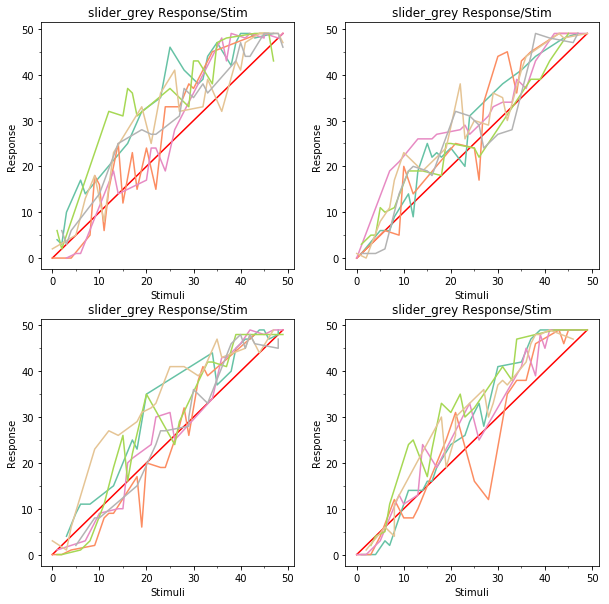
\includegraphics[width=1.1\textwidth]{figures/visual_out1.png}
\caption{Visualization of outliers for the arm\_grey exercise}
\label{NAN}
\end{figure}

\begin{figure}[h!]
\centering
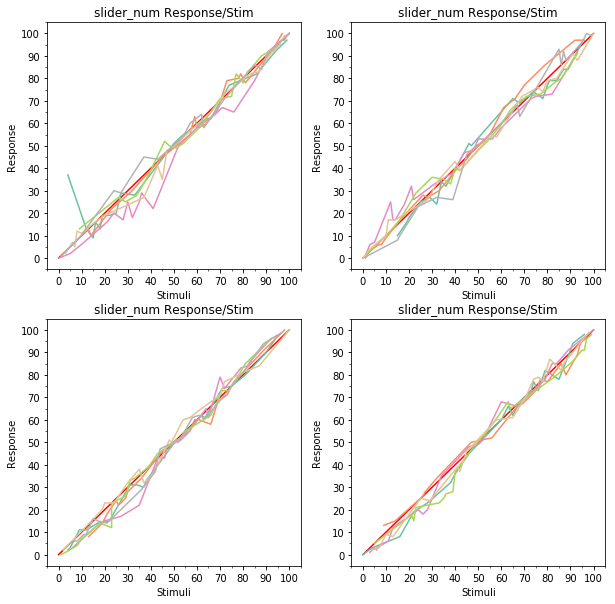
\includegraphics[width=1.1\textwidth]{figures/visual_out2.png}
\caption{Visualization of outliers for the arm\_grey exercise}
\label{NAN}
\end{figure}

\begin{figure}[h!]
\centering
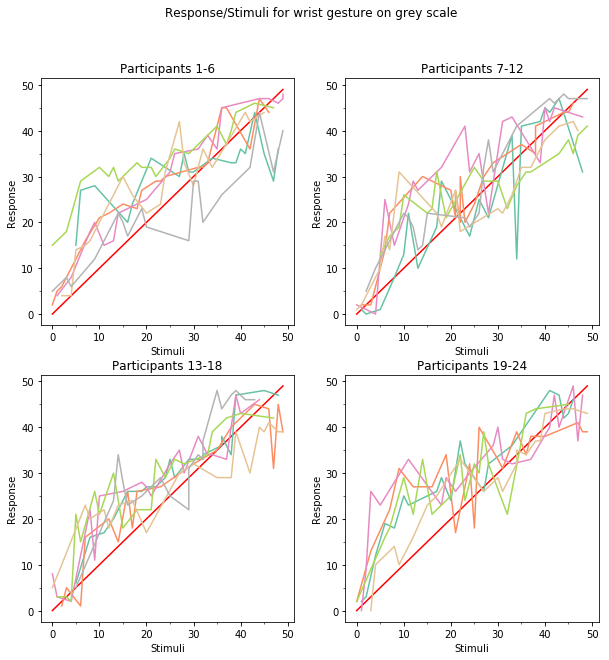
\includegraphics[width=1.1\textwidth]{figures/visual_out3.png}
\caption{Visualization of outliers for the arm\_grey exercise}
\label{NAN}
\end{figure}

\begin{figure}[h!]
\centering
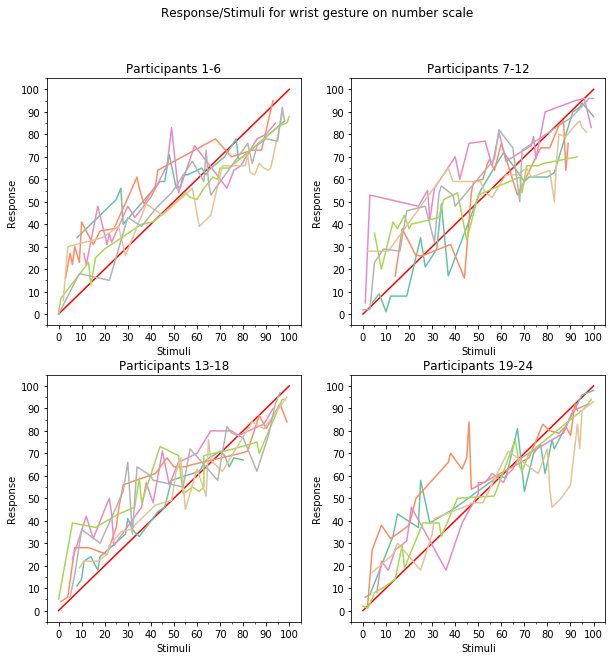
\includegraphics[width=1.1\textwidth]{figures/visual_out4.png}
\caption{Visualization of outliers for the arm\_grey exercise}
\label{NAN}
\end{figure}

\begin{figure}[h!]
\centering
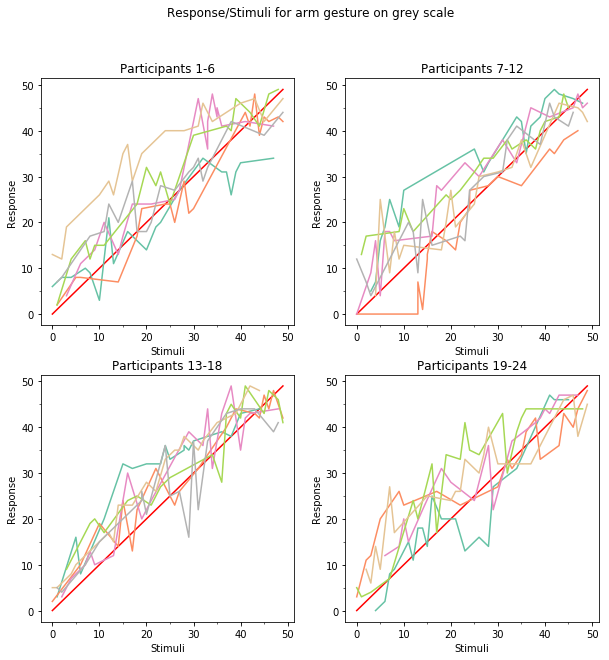
\includegraphics[width=1.1\textwidth]{figures/visual_out5.png}
\caption{Visualization of outliers for the arm\_grey exercise}
\label{NAN}
\end{figure}

\begin{figure}[h!]
\centering
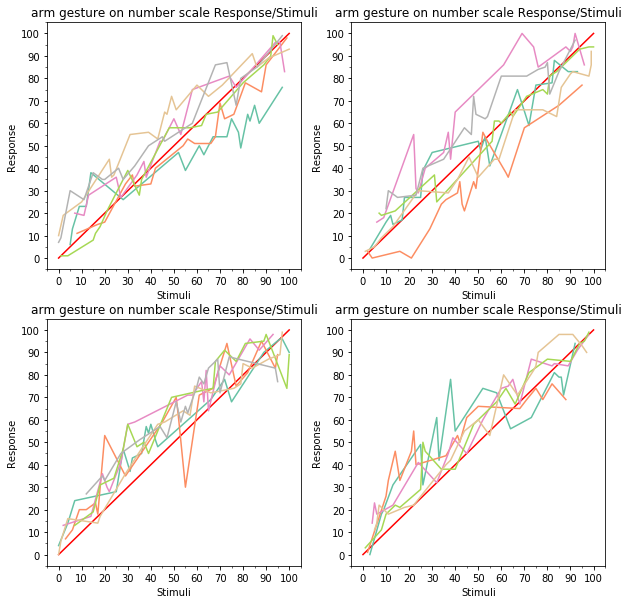
\includegraphics[width=1.1\textwidth]{figures/visual_out6.png}
\caption{Visualization of outliers for the arm\_grey exercise}
\label{NAN}
\end{figure}













\chapter{Experiment App Screens}\label{ex_app_screens}
\begin{figure}[h!]
\centering
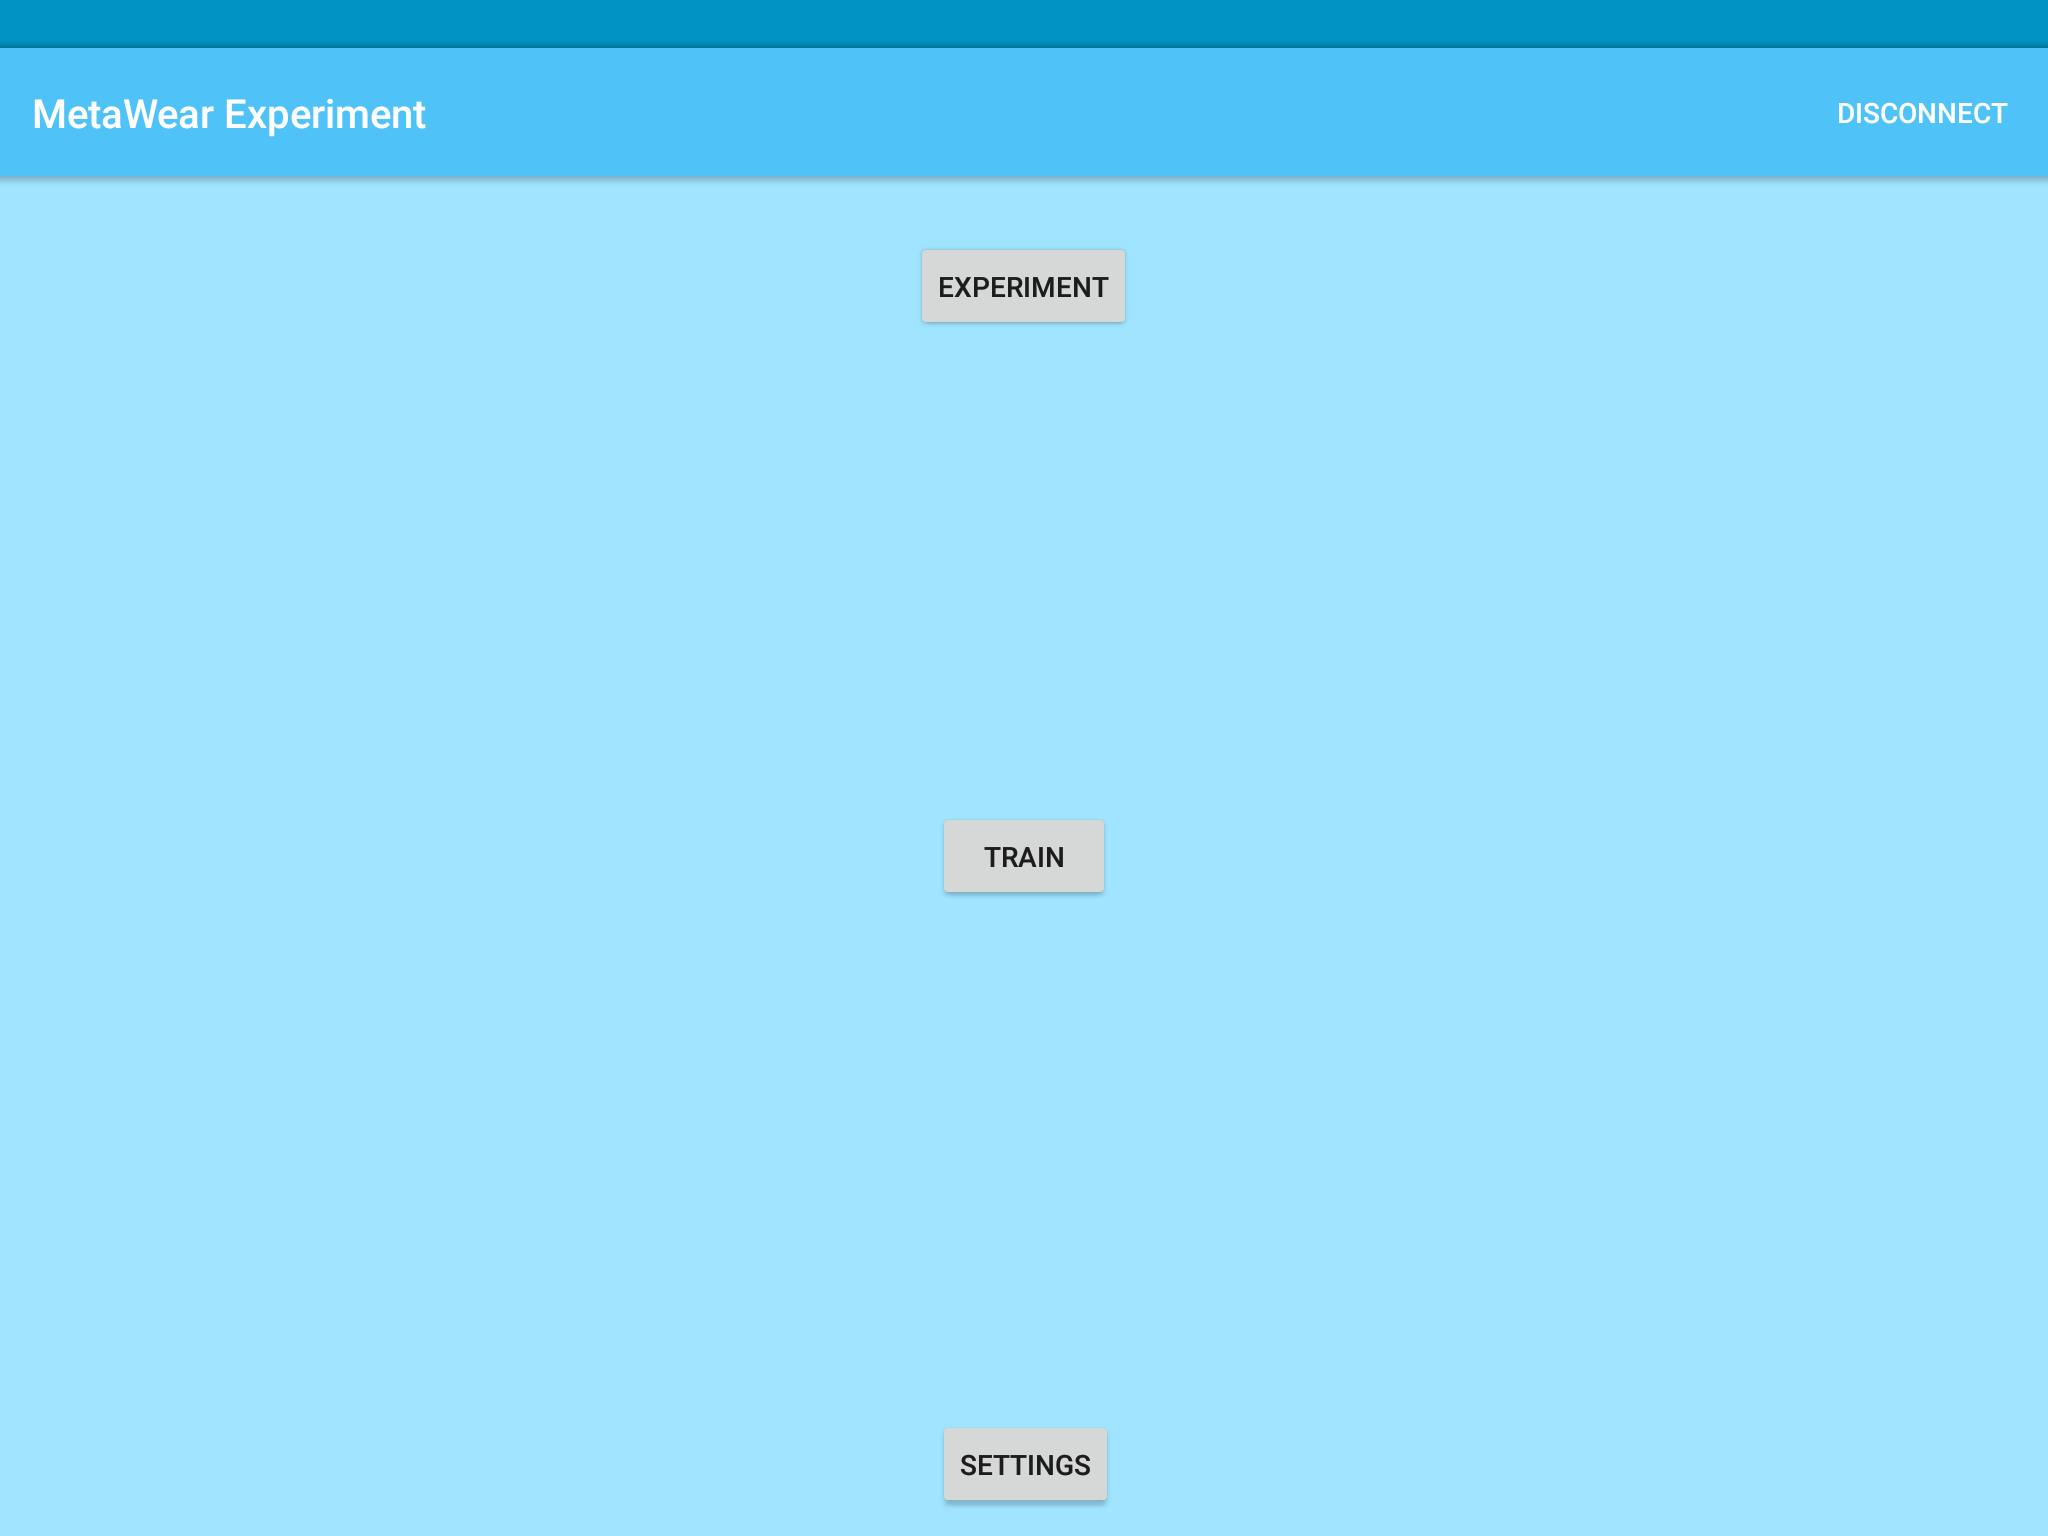
\includegraphics[width=0.9\textwidth]{figures/tablet_screen0.png}
\caption{CAPTIONBLABLA}
\label{appendix_app_screen_0}
\end{figure}

\begin{figure}[h!]
\centering
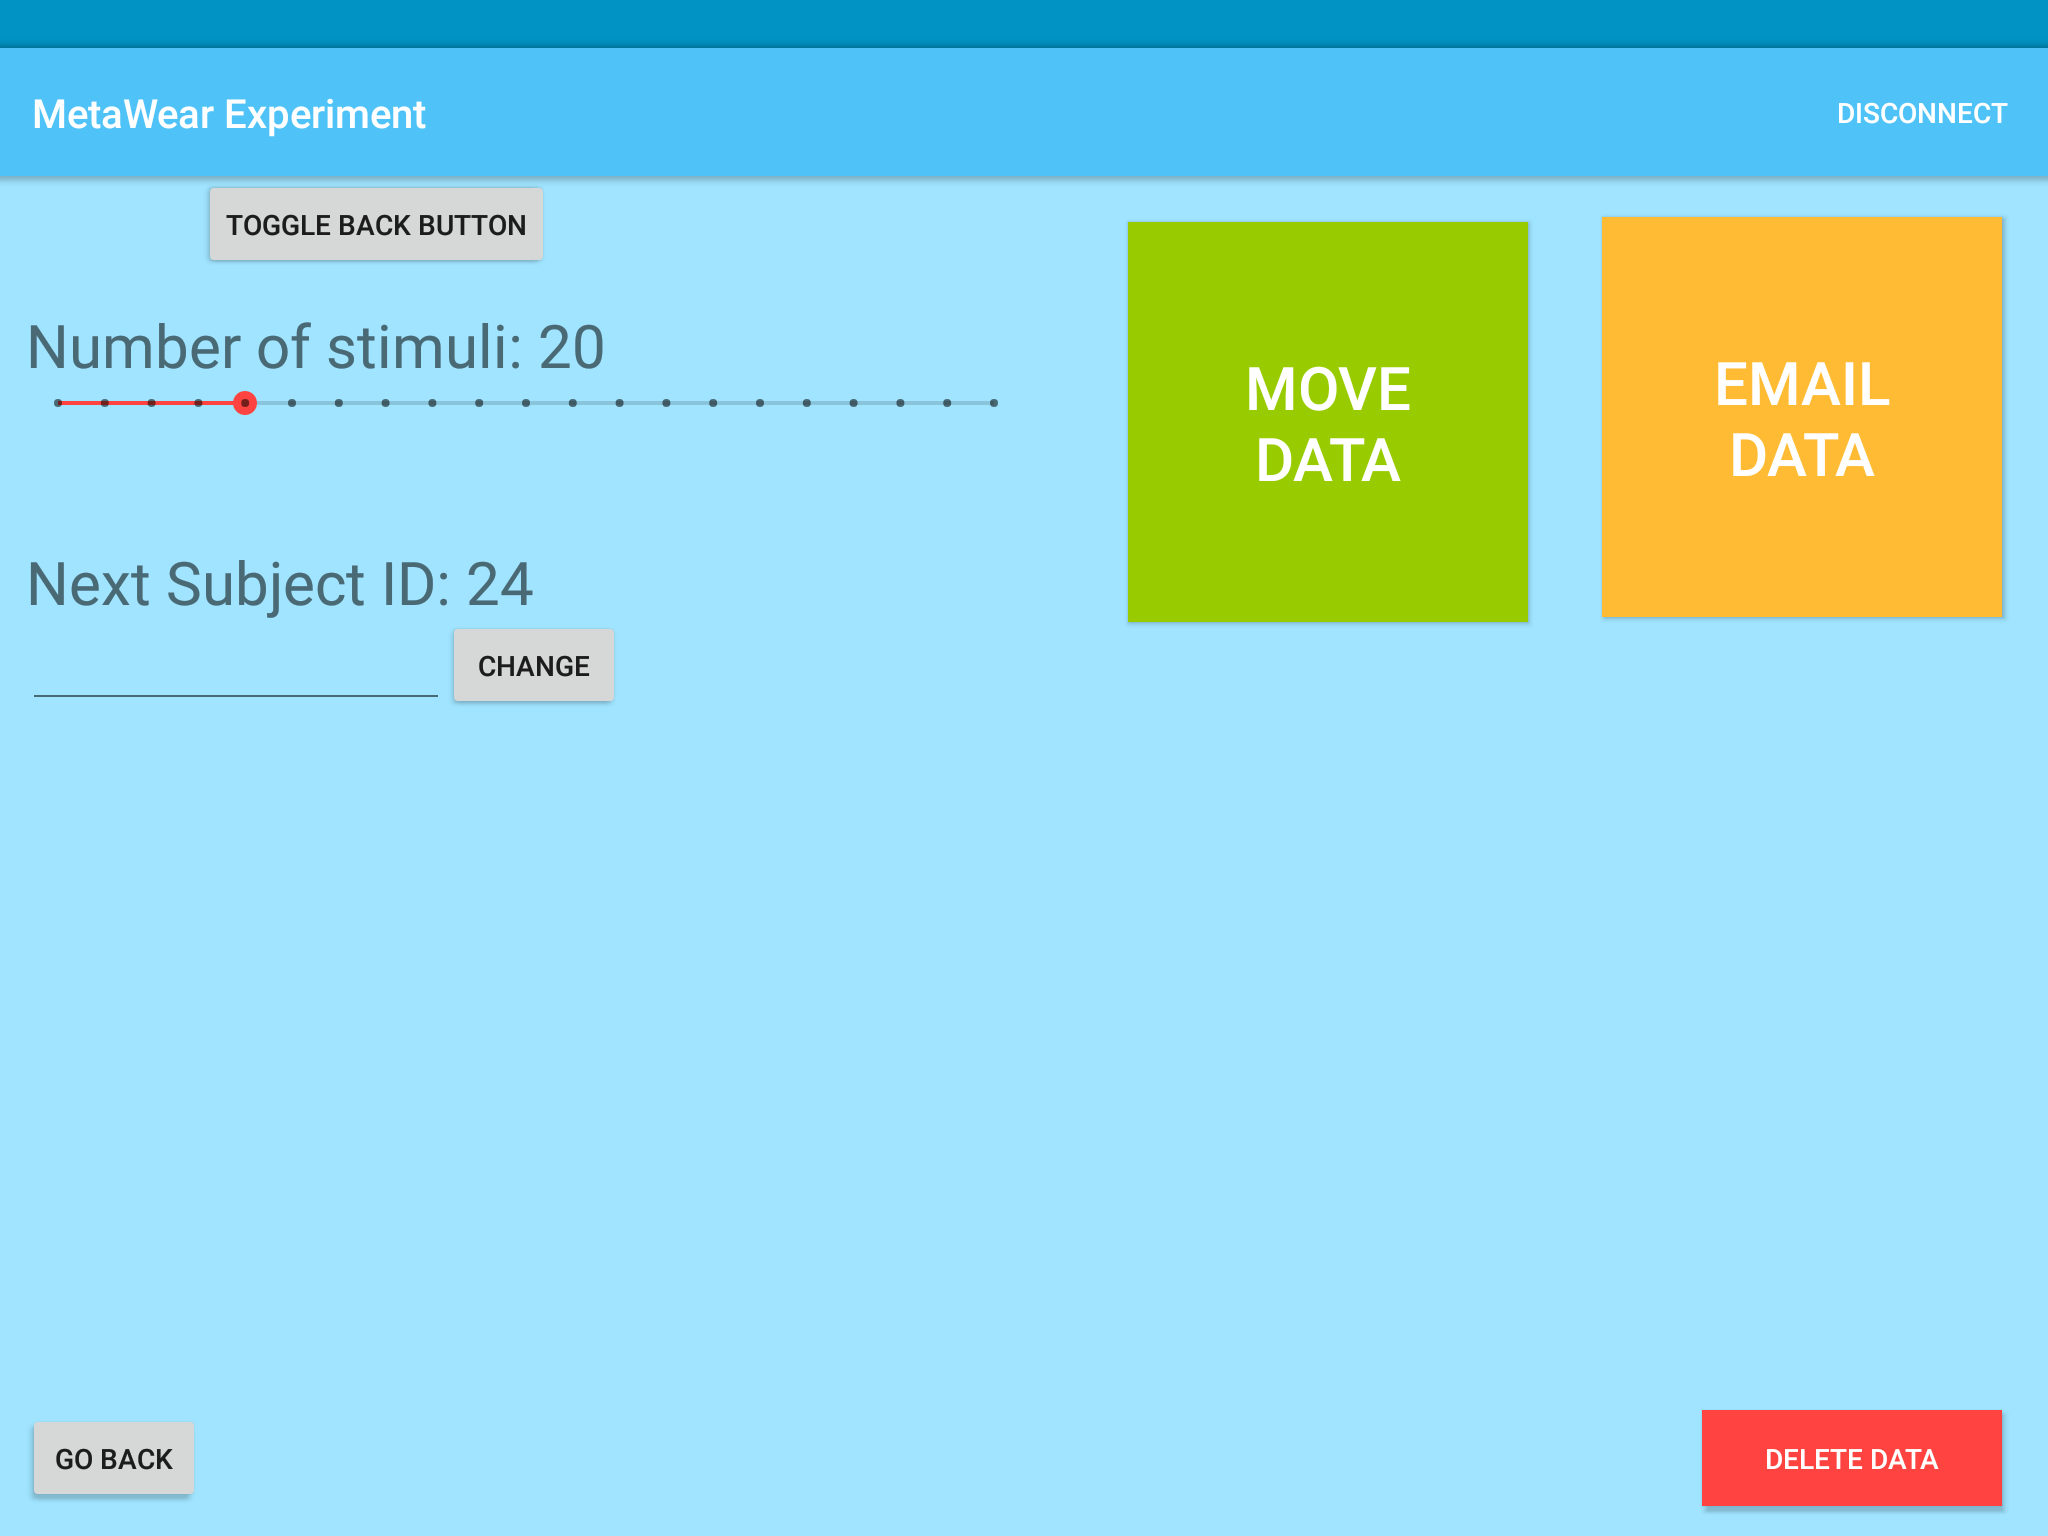
\includegraphics[width=0.9\textwidth]{figures/tablet_screen1.png}
\caption{CAPTIONBLABLA}
\label{appendix_app_screen_1}
\end{figure}

\begin{figure}[h!]
\centering
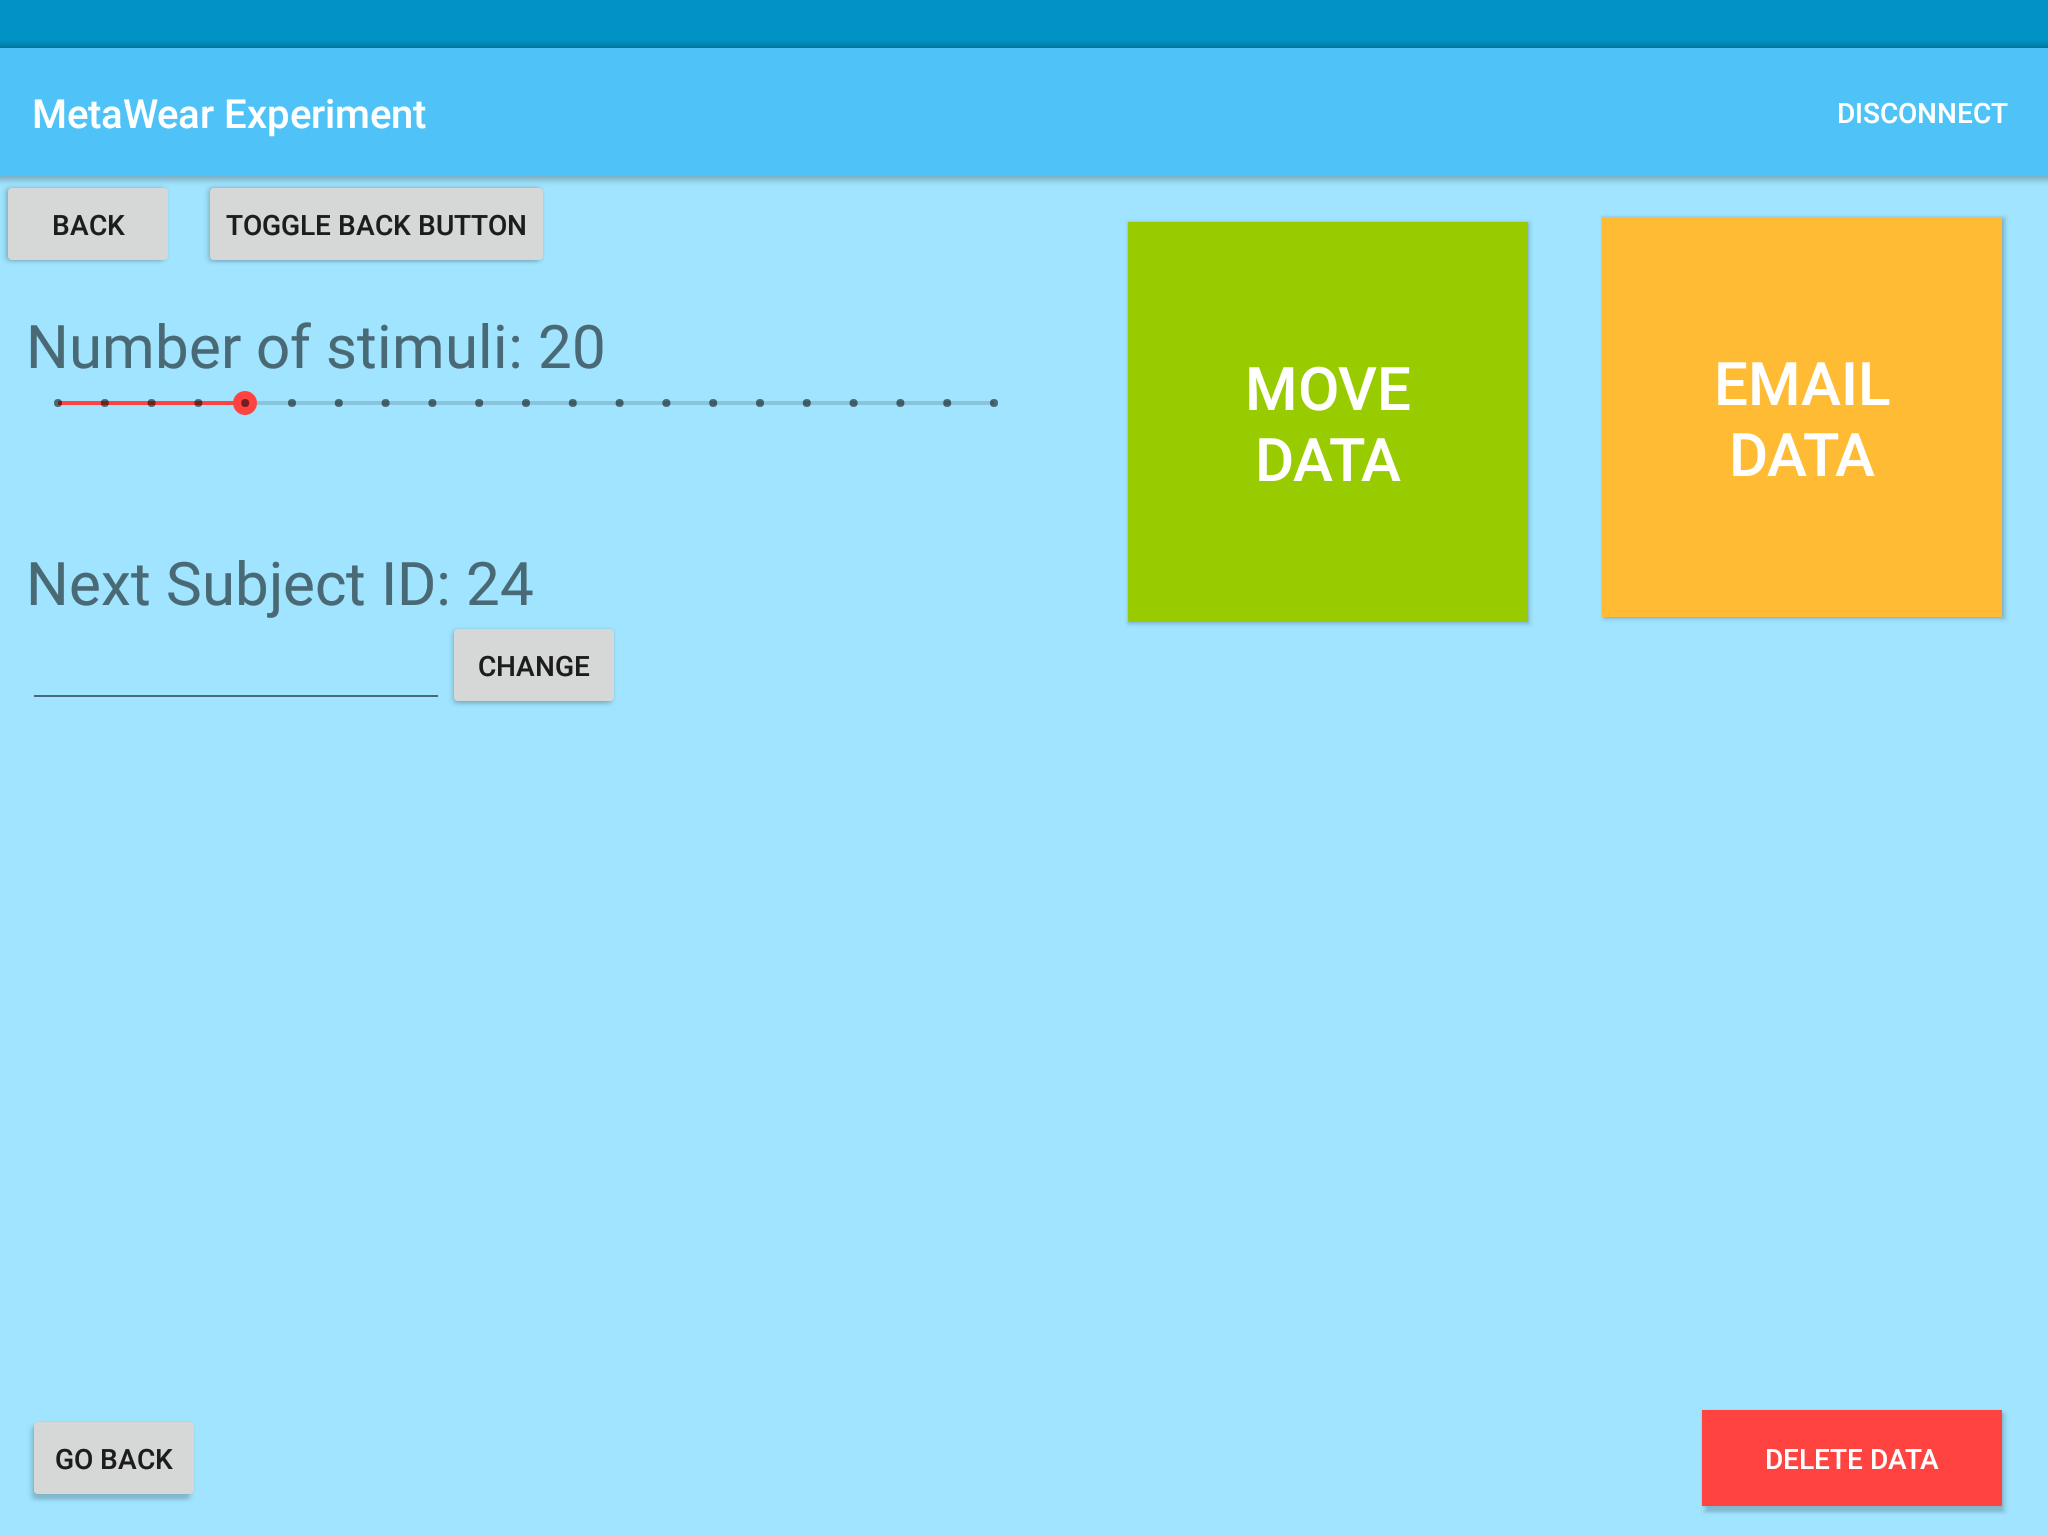
\includegraphics[width=0.9\textwidth]{figures/tablet_screen2.png}
\caption{CAPTIONBLABLA}
\label{appendix_app_screen_2}
\end{figure}

\begin{figure}[h!]
\centering
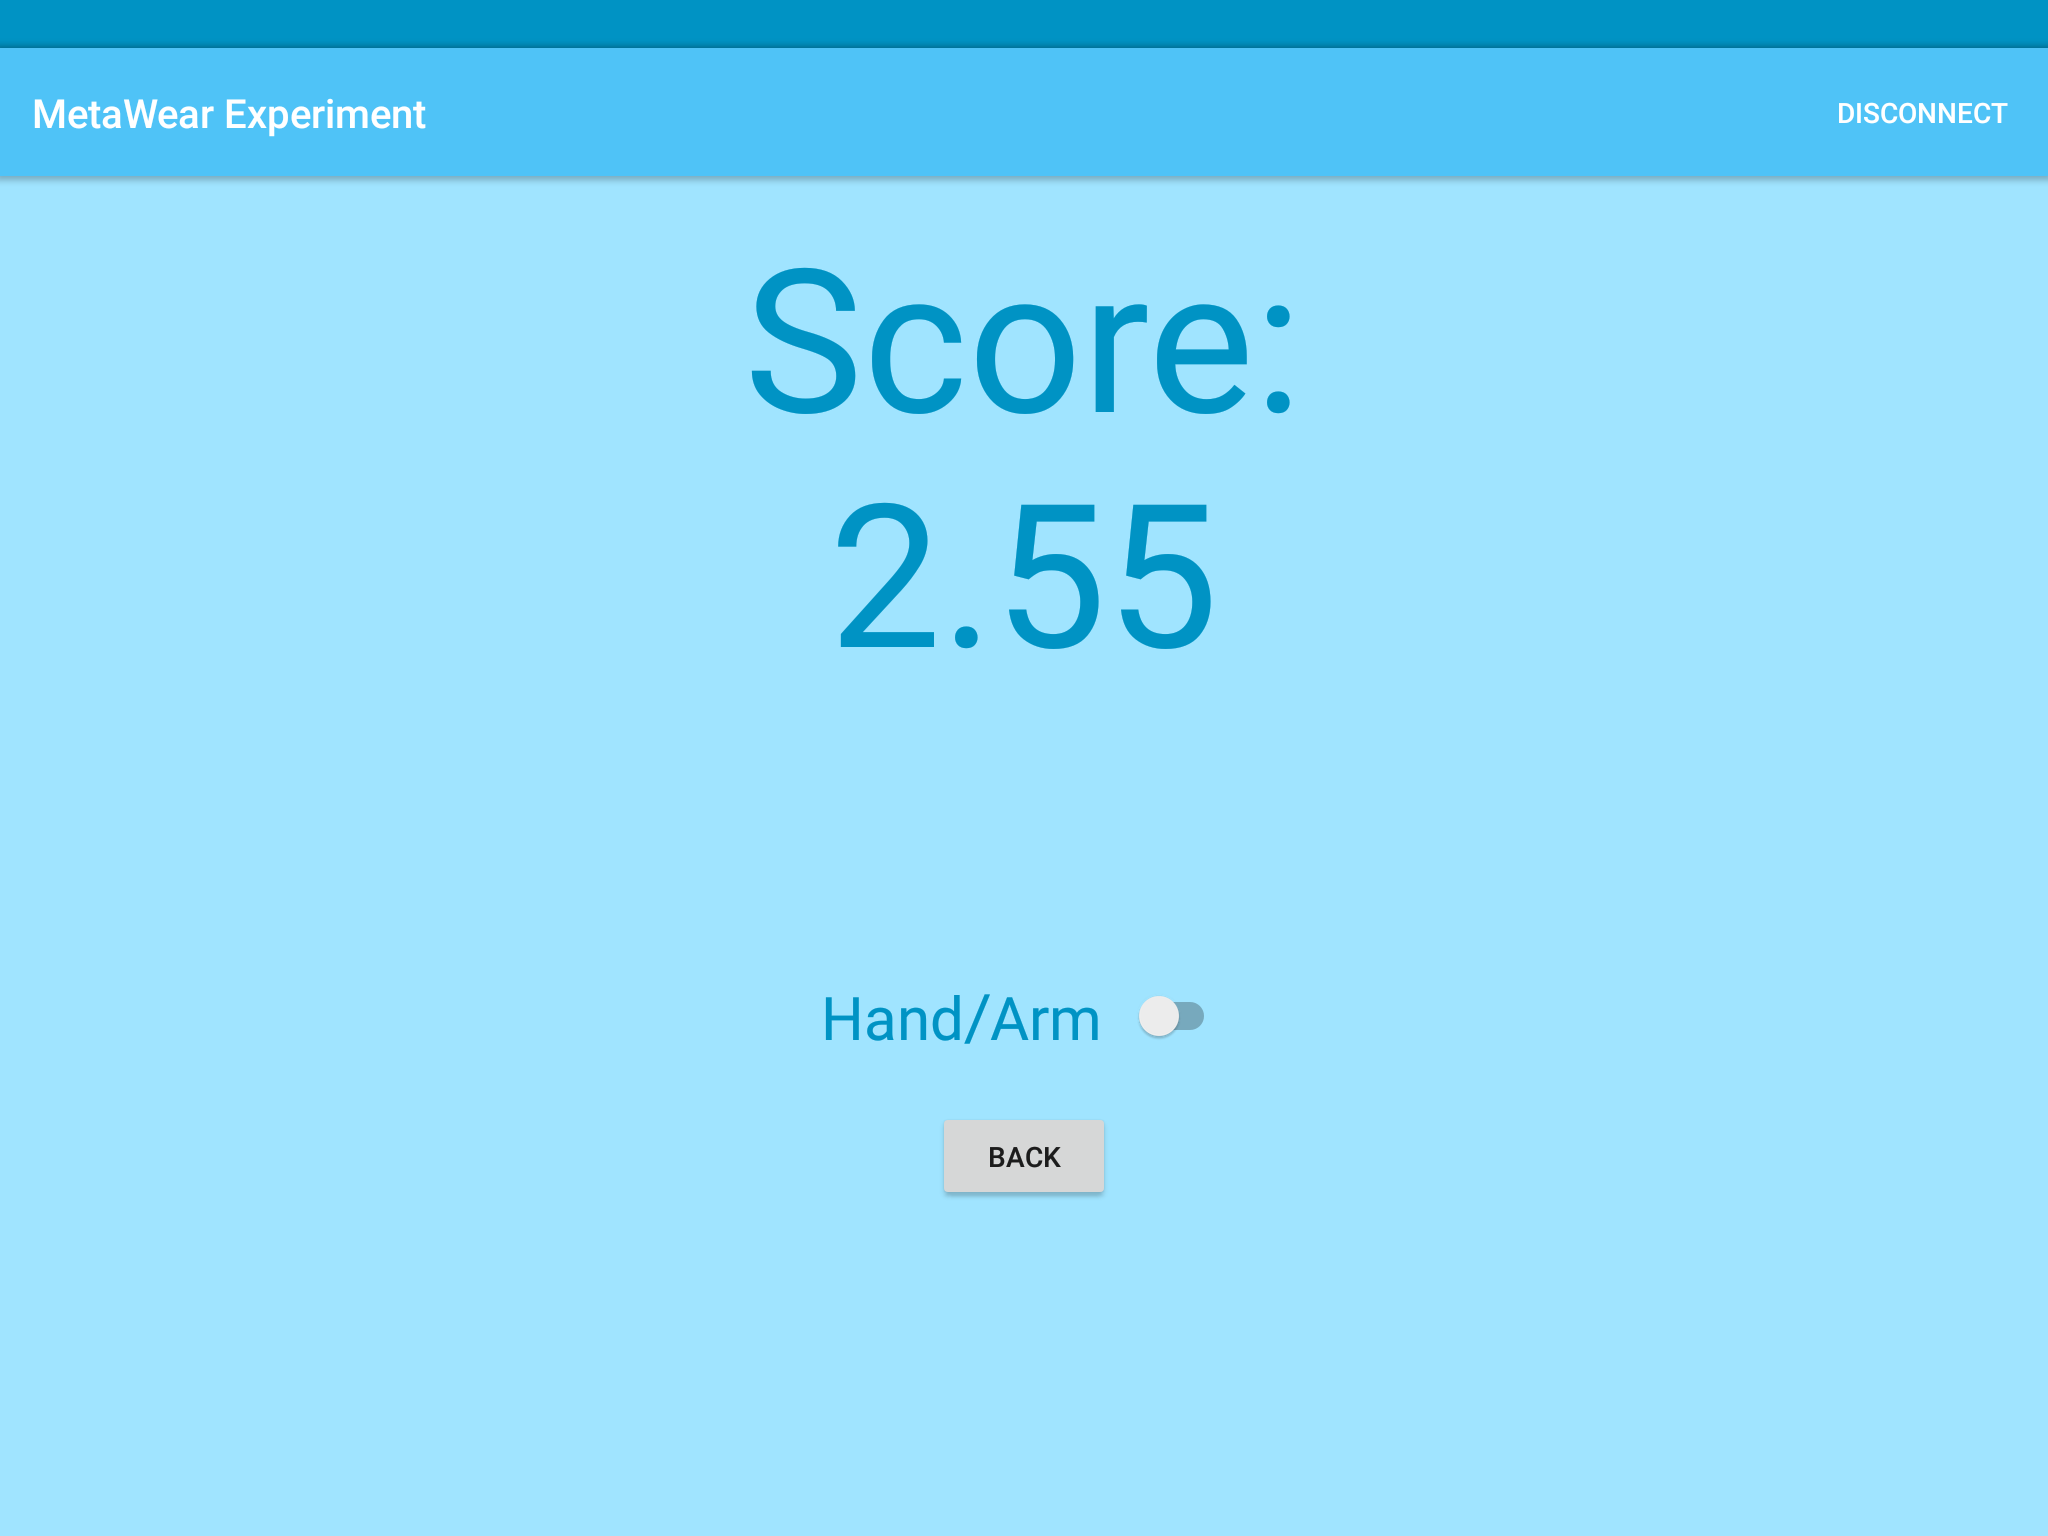
\includegraphics[width=0.9\textwidth]{figures/tablet_screen3.png}
\caption{CAPTIONBLABLA}
\label{appendix_app_screen_3}
\end{figure}

\begin{figure}[h!]
\centering
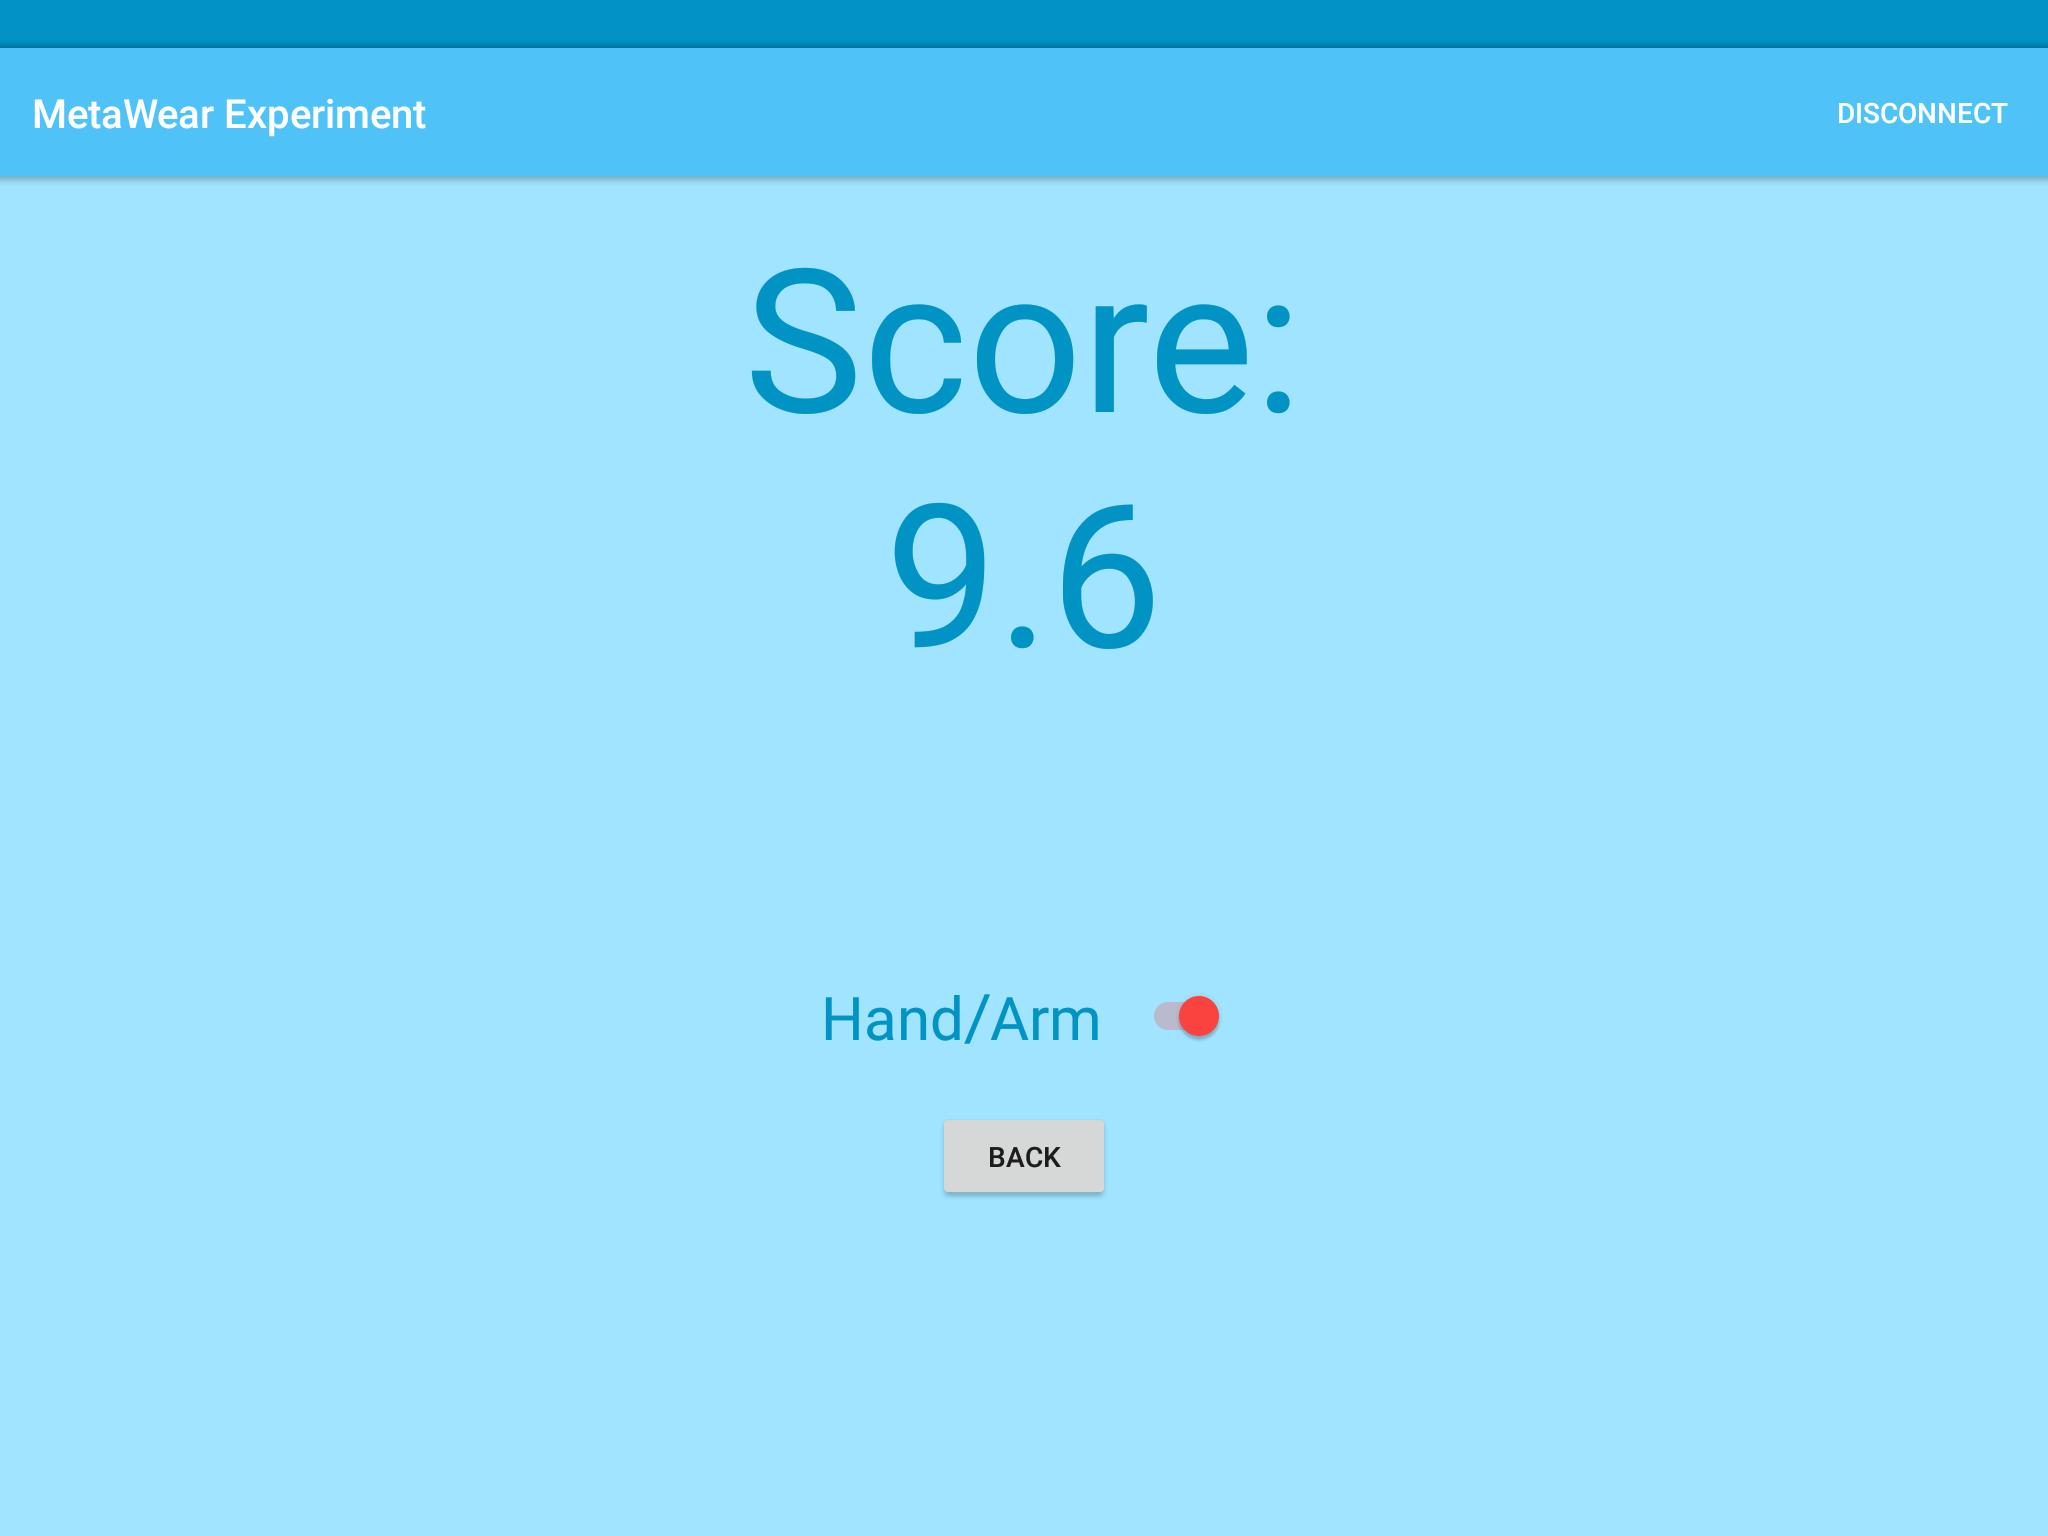
\includegraphics[width=0.9\textwidth]{figures/tablet_screen4.png}
\caption{CAPTIONBLABLA}
\label{appendix_app_screen_4}
\end{figure}

\begin{figure}[h!]
\centering
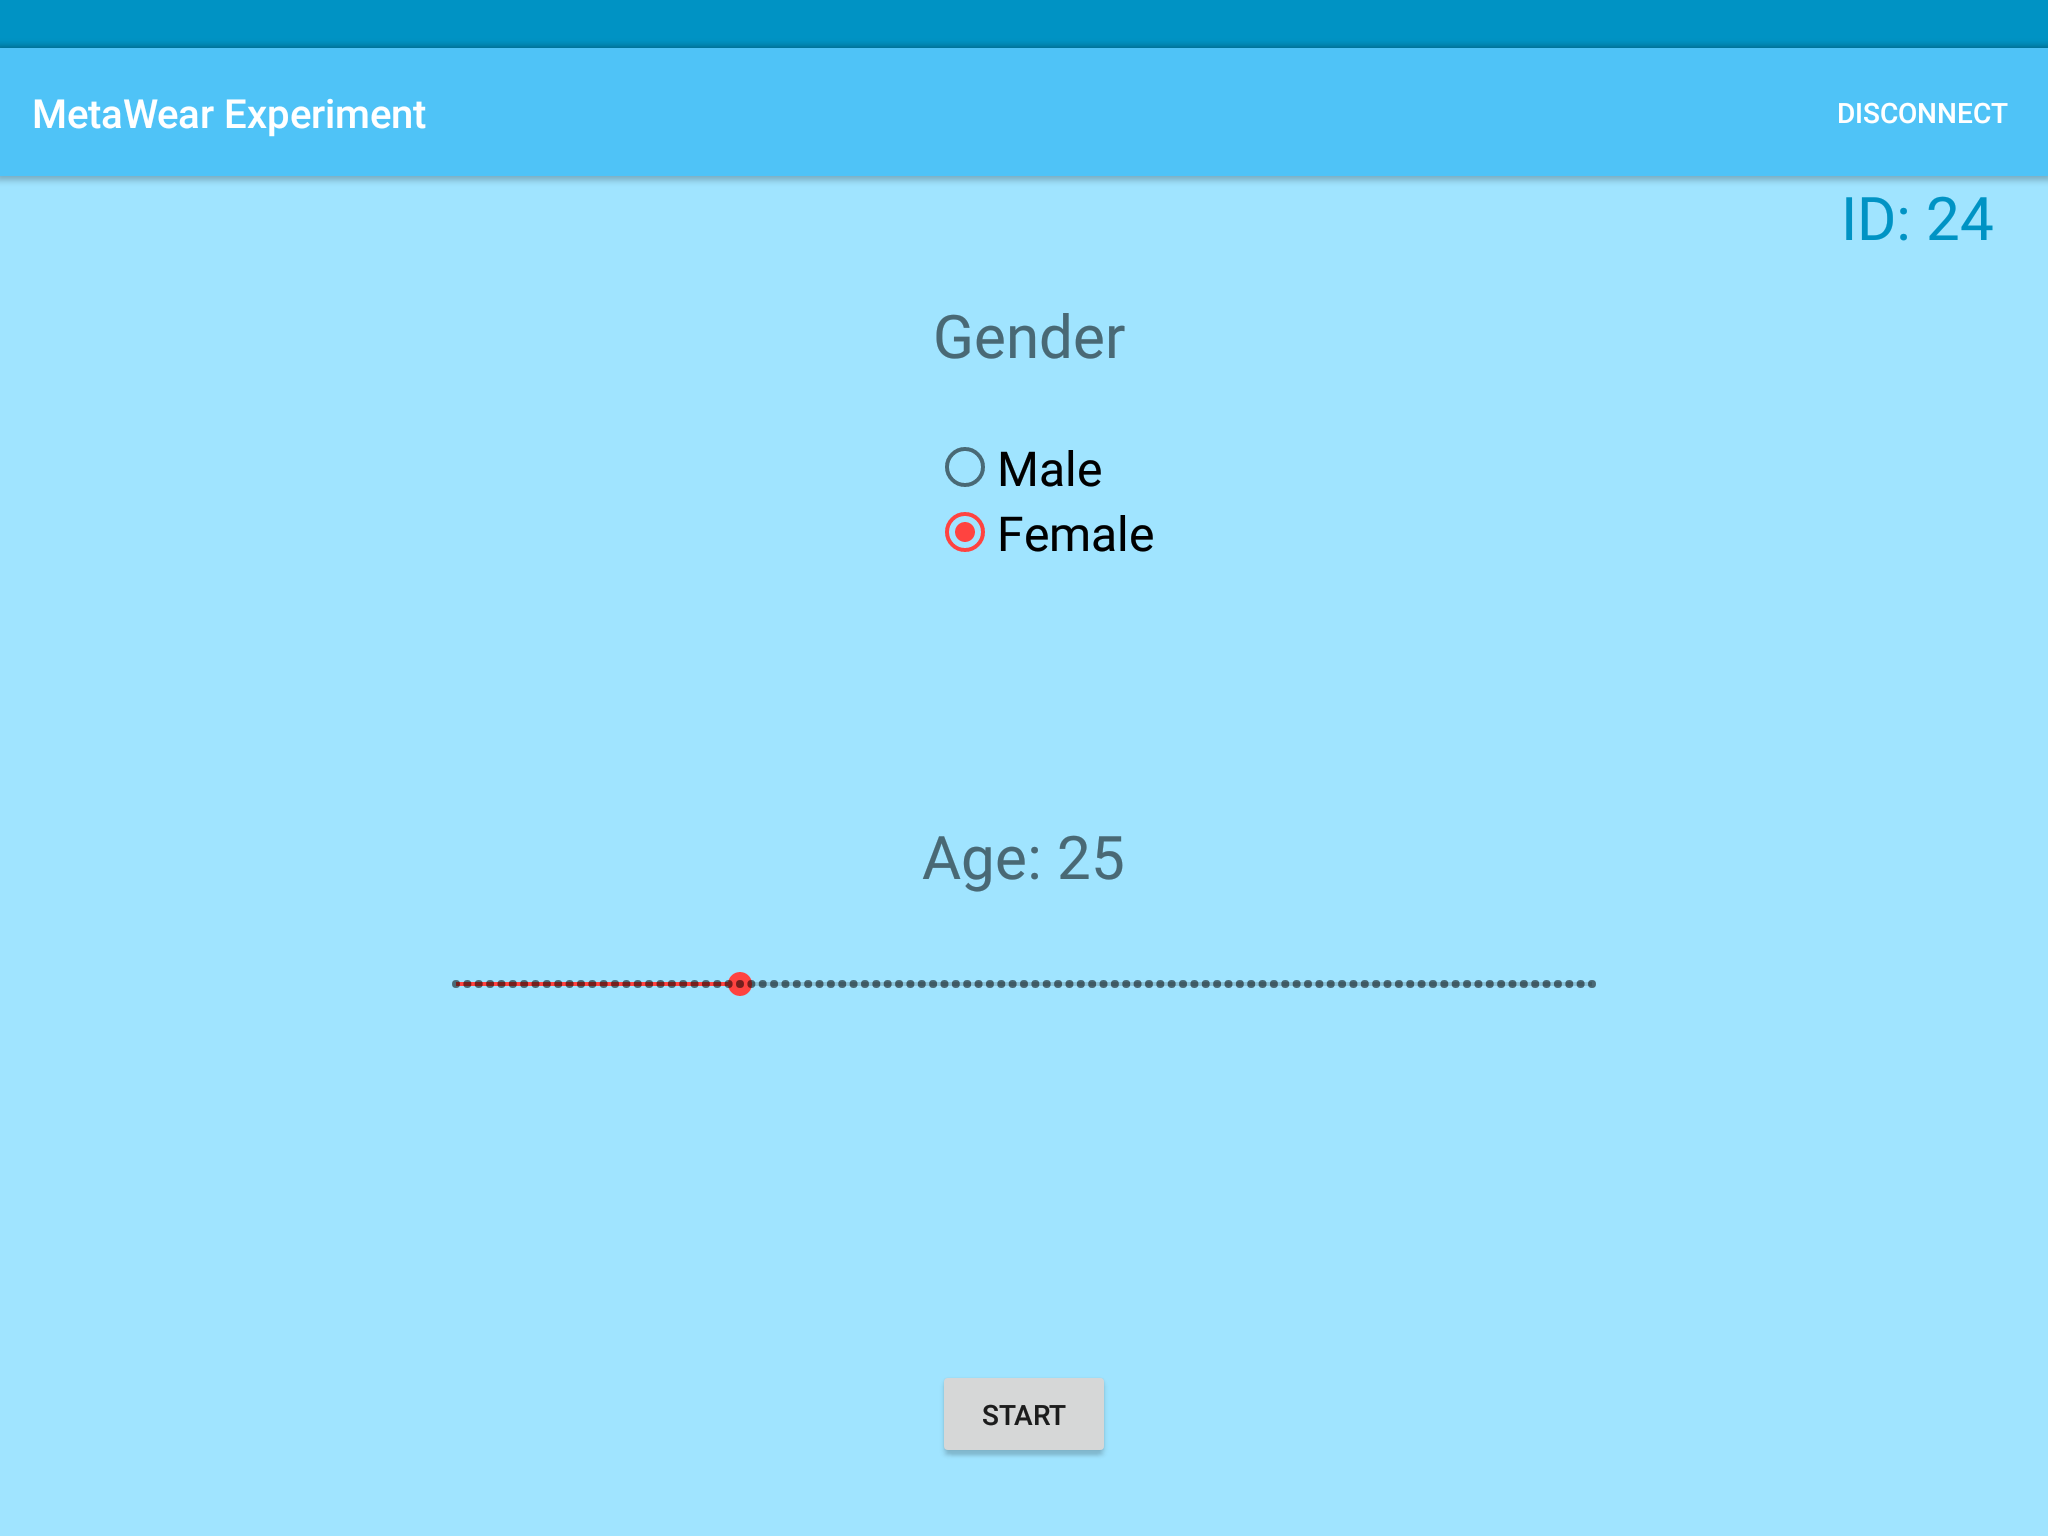
\includegraphics[width=0.9\textwidth]{figures/tablet_screen5.png}
\caption{CAPTIONBLABLA}
\label{appendix_app_screen_5}
\end{figure}

\begin{figure}[h!]
\centering
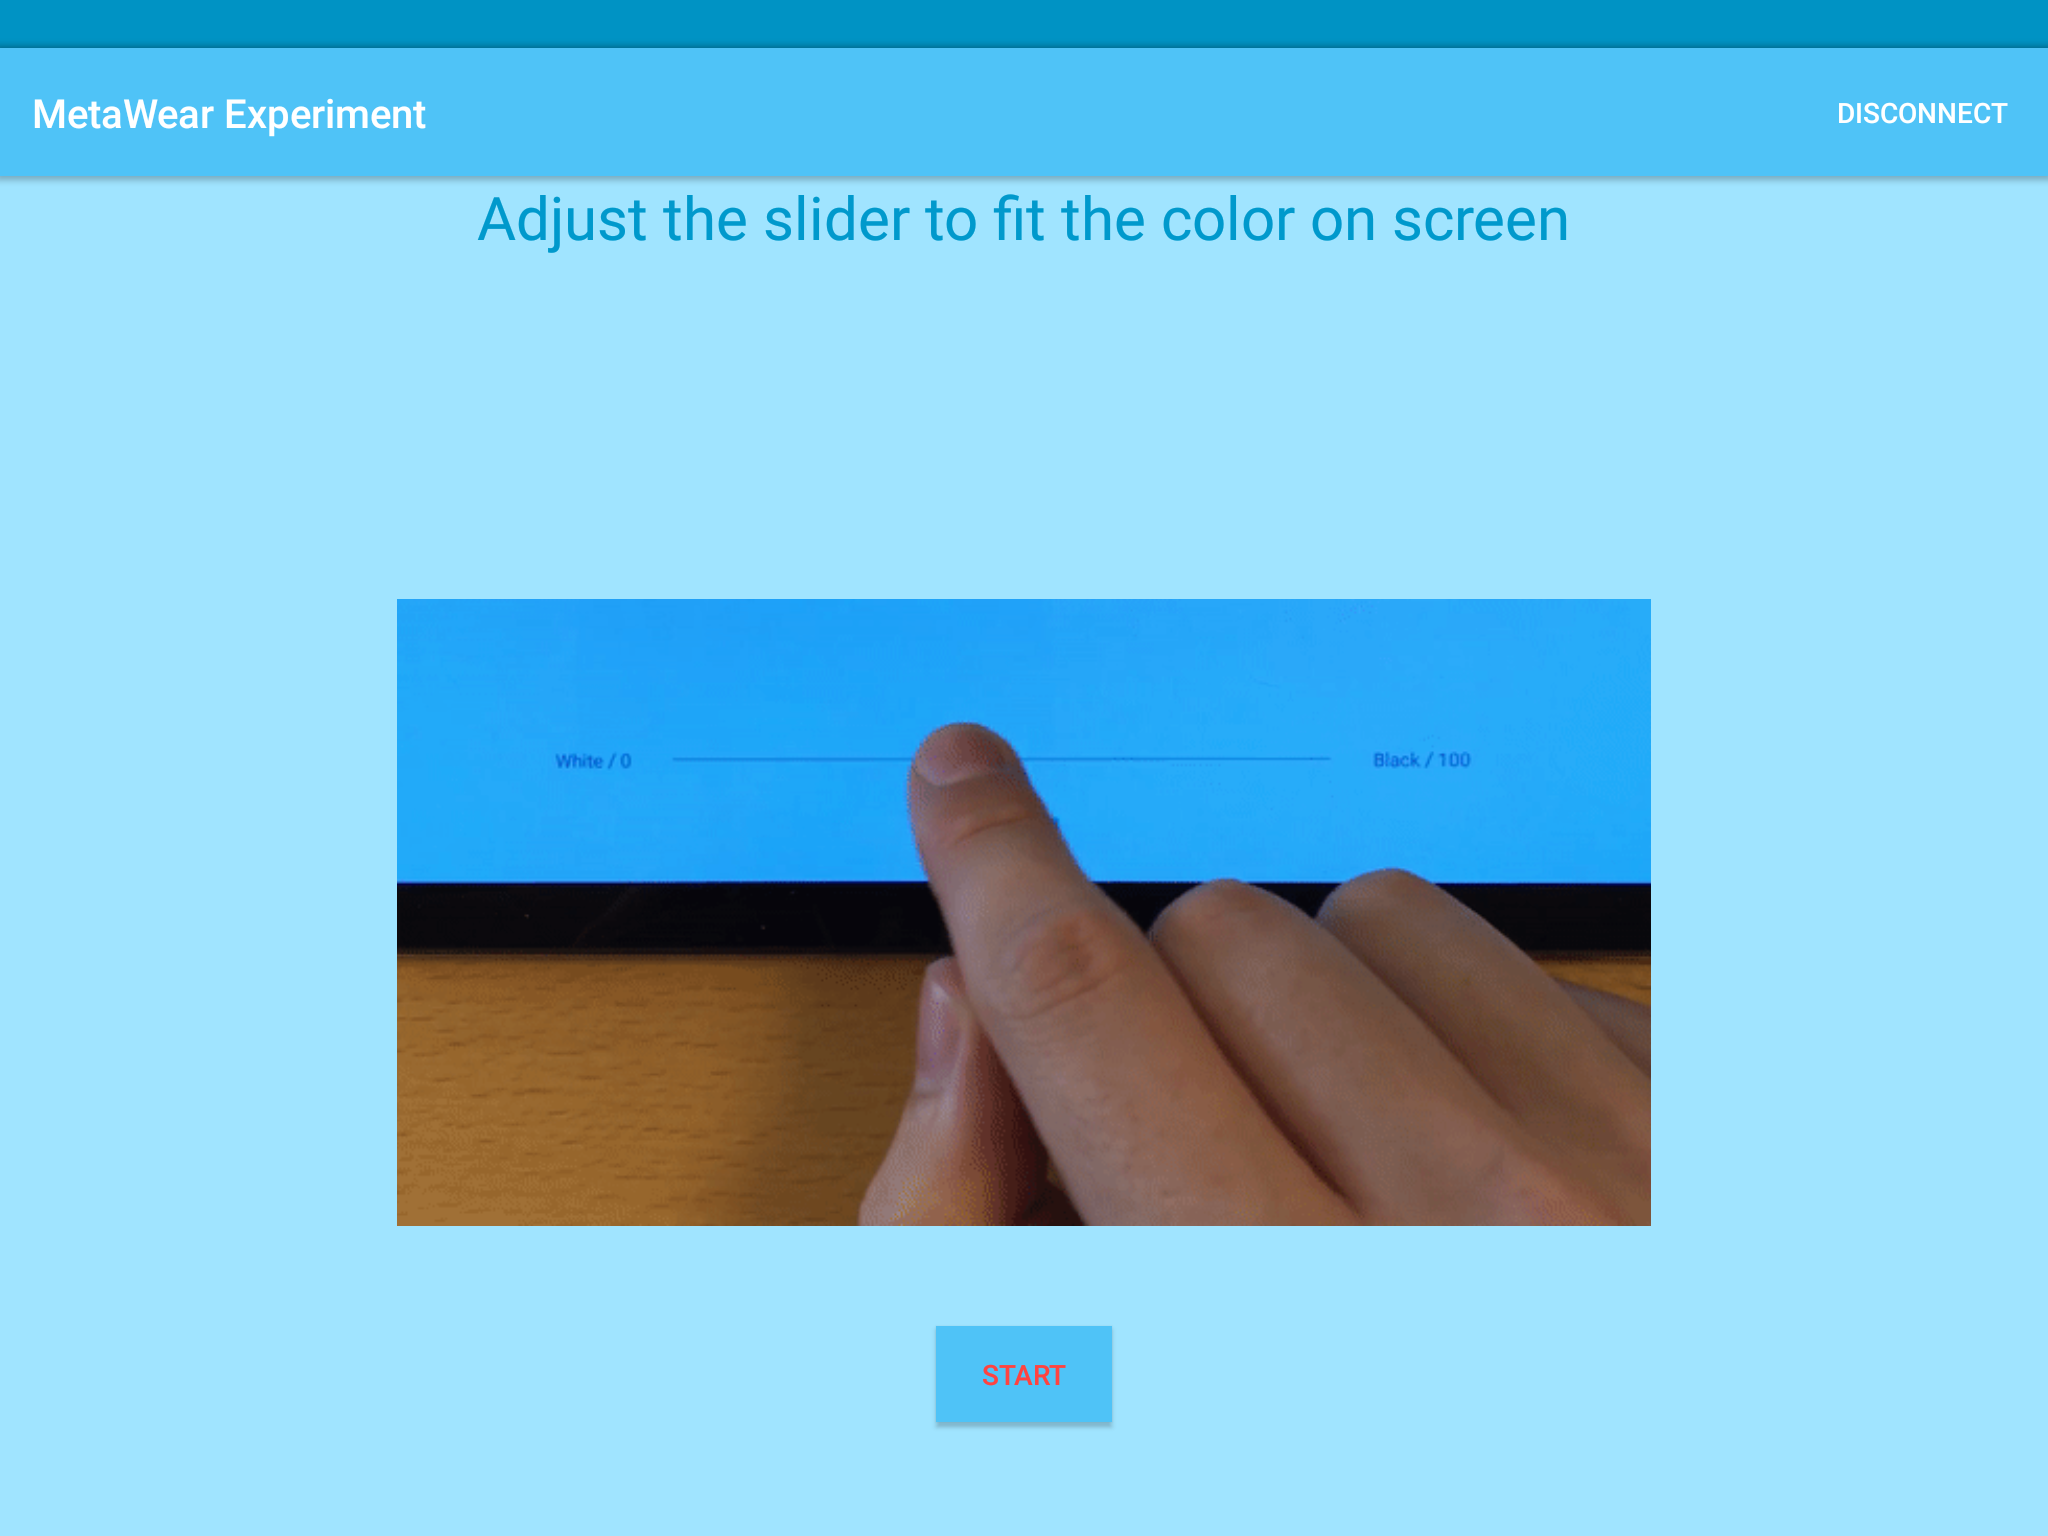
\includegraphics[width=0.9\textwidth]{figures/tablet_screen6.png}
\caption{CAPTIONBLABLA}
\label{appendix_app_screen_6}
\end{figure}

\begin{figure}[h!]
\centering
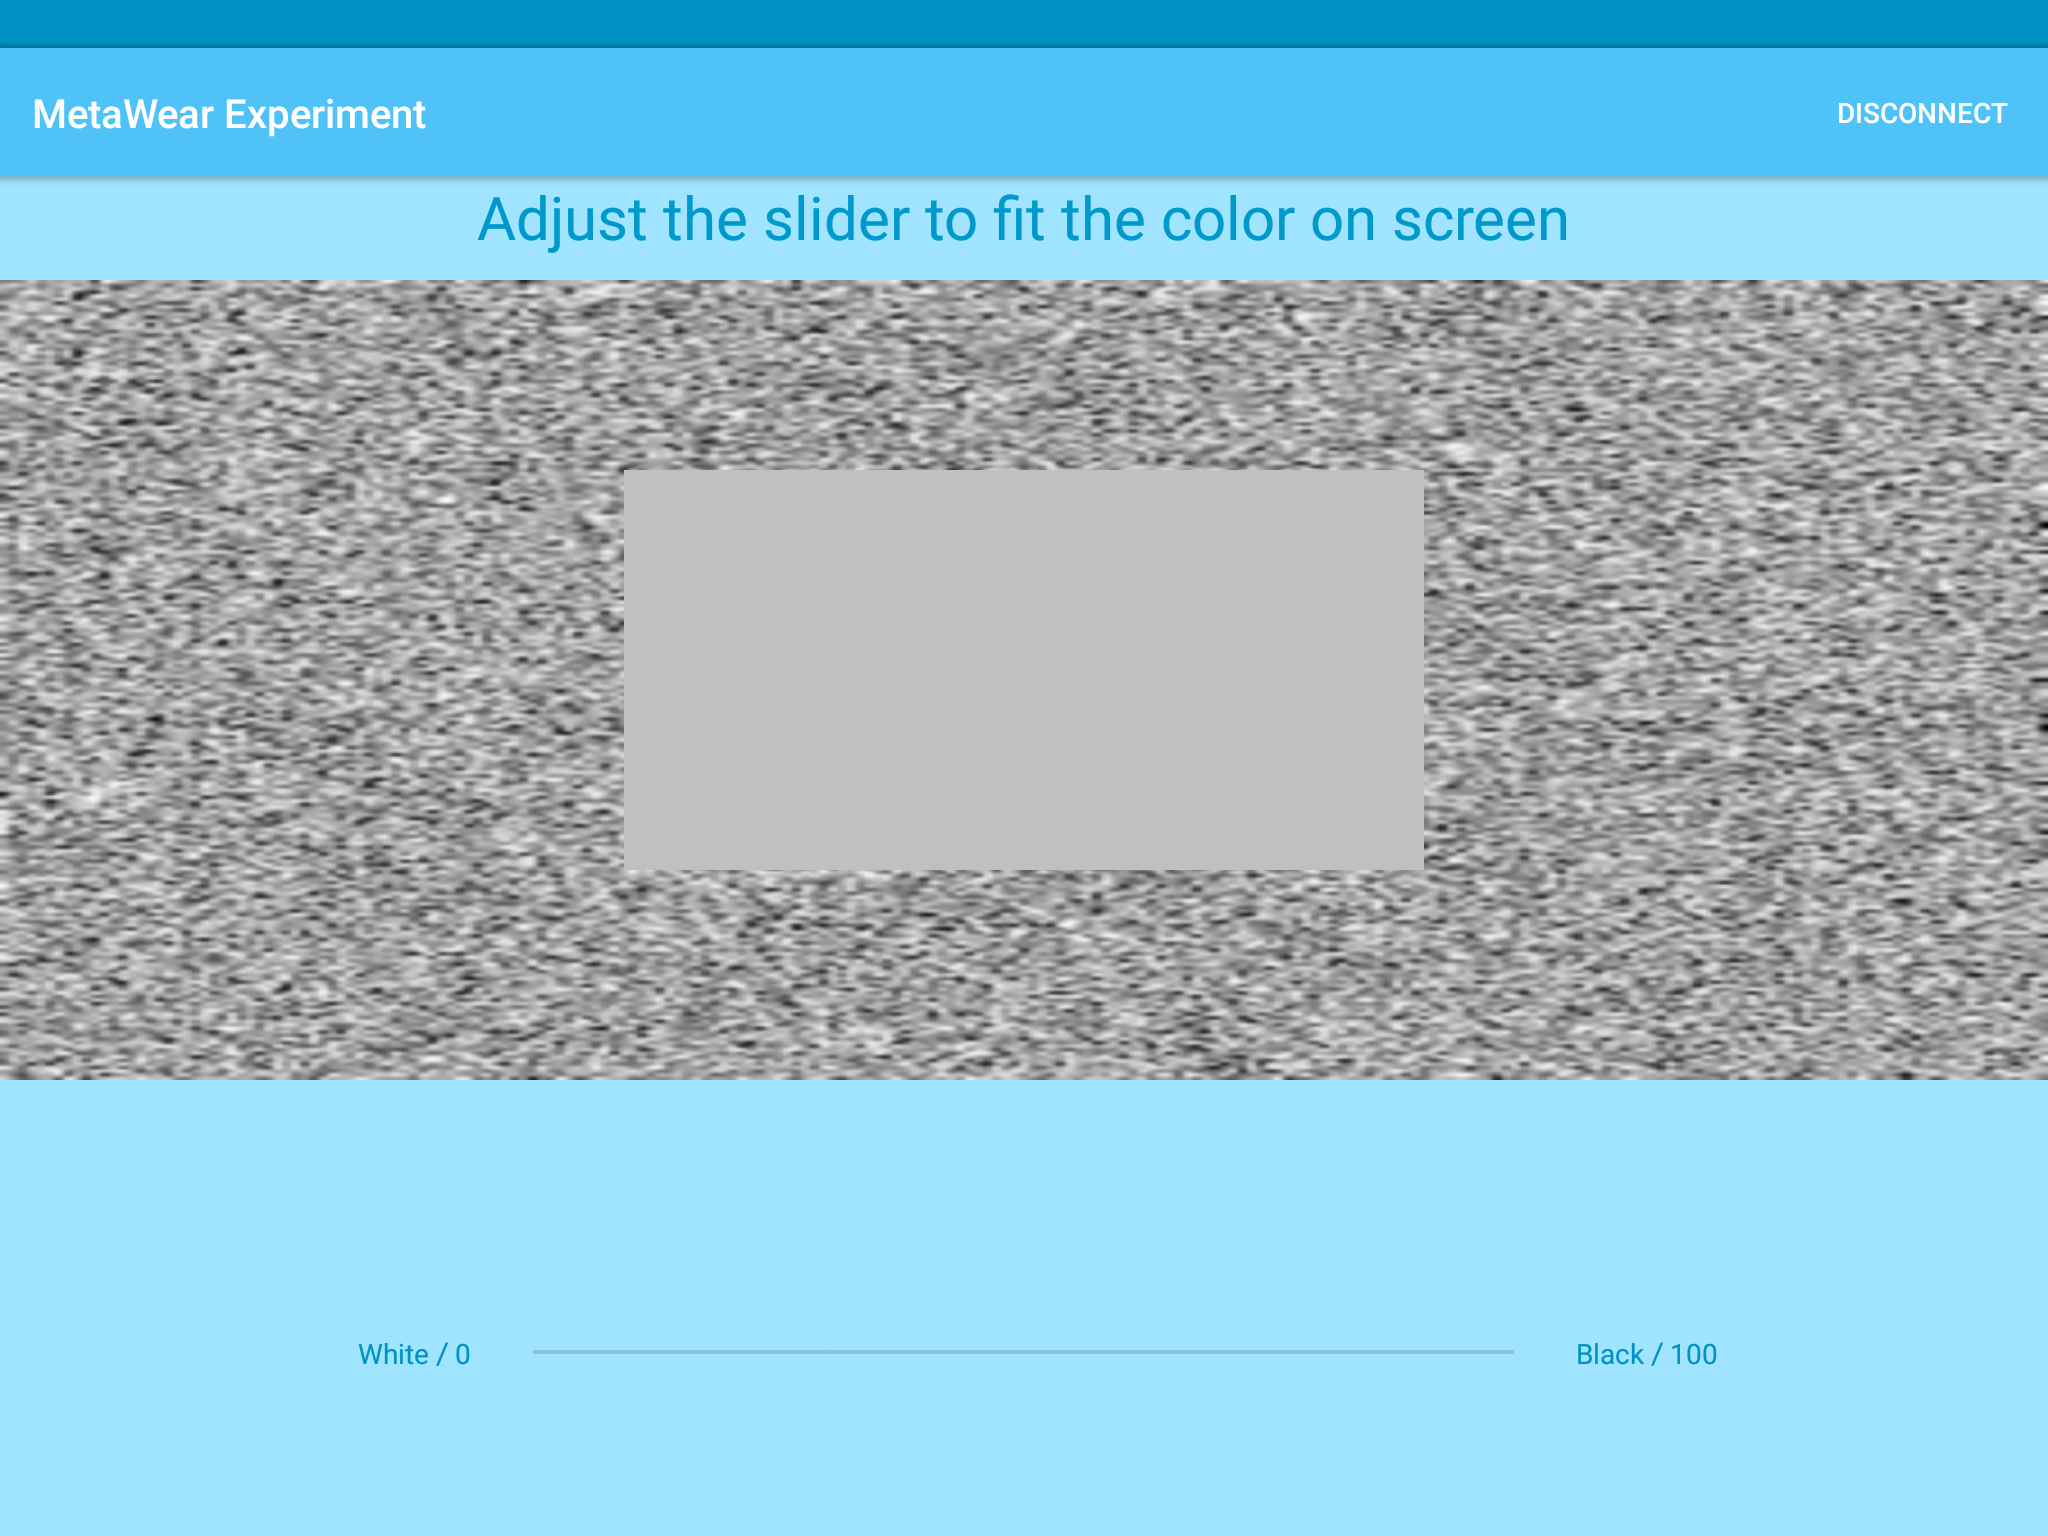
\includegraphics[width=0.9\textwidth]{figures/tablet_screen7.png}
\caption{CAPTIONBLABLA}
\label{appendix_app_screen_7}
\end{figure}

\begin{figure}[h!]
\centering
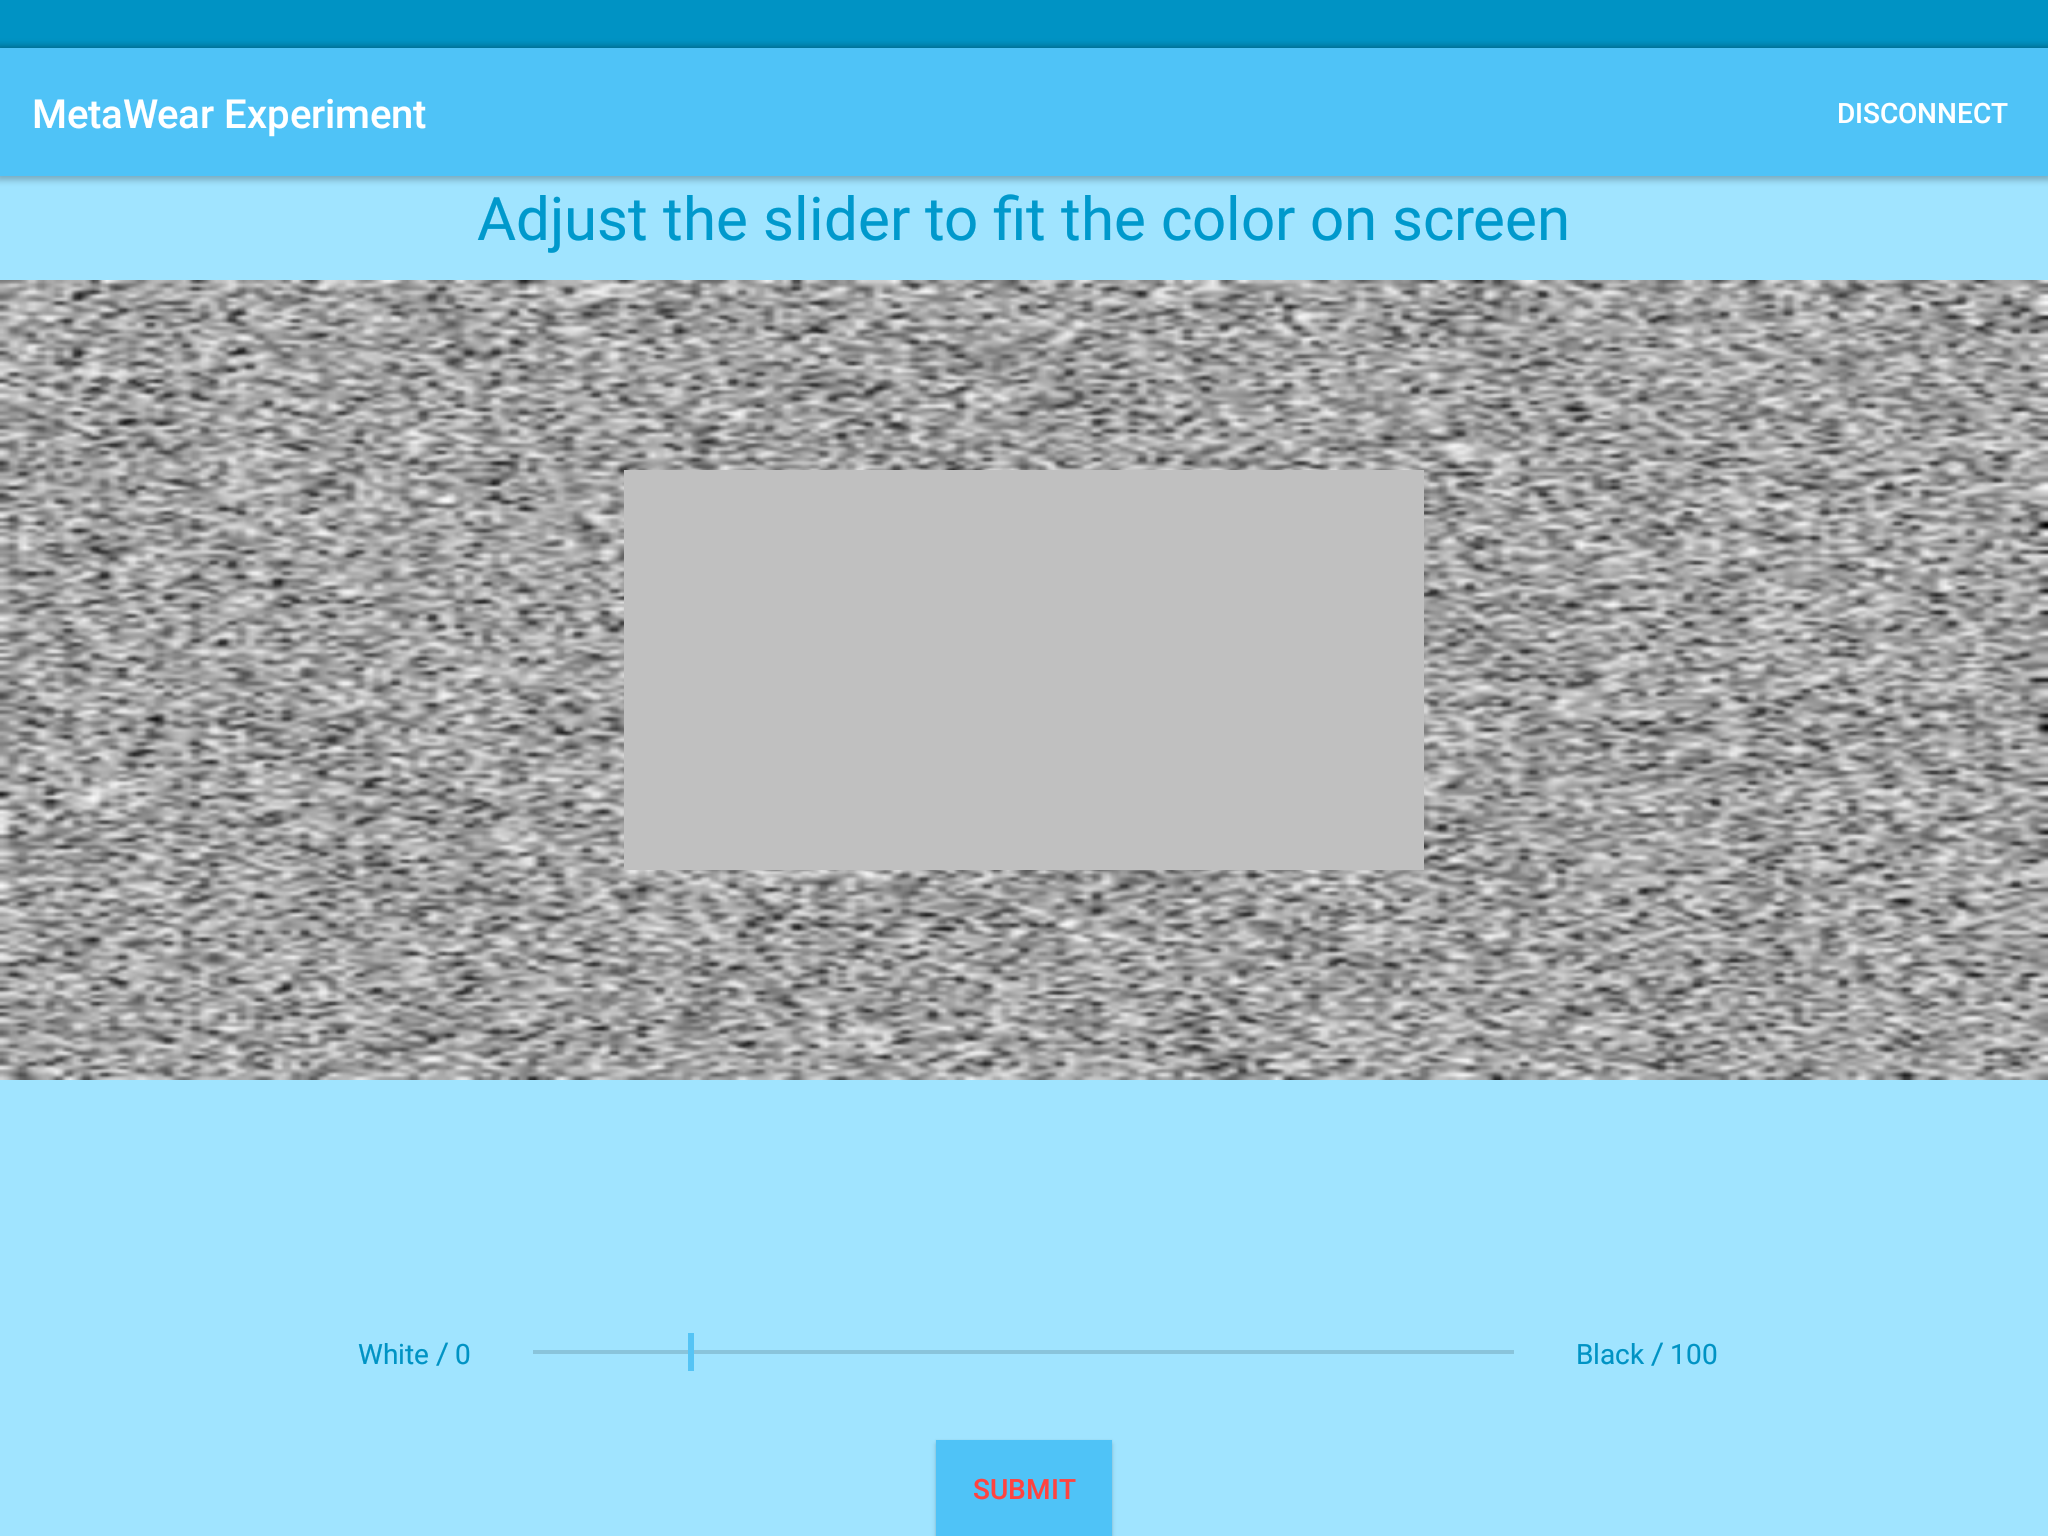
\includegraphics[width=0.9\textwidth]{figures/tablet_screen8.png}
\caption{CAPTIONBLABLA}
\label{appendix_app_screen_8}
\end{figure}

\begin{figure}[h!]
\centering
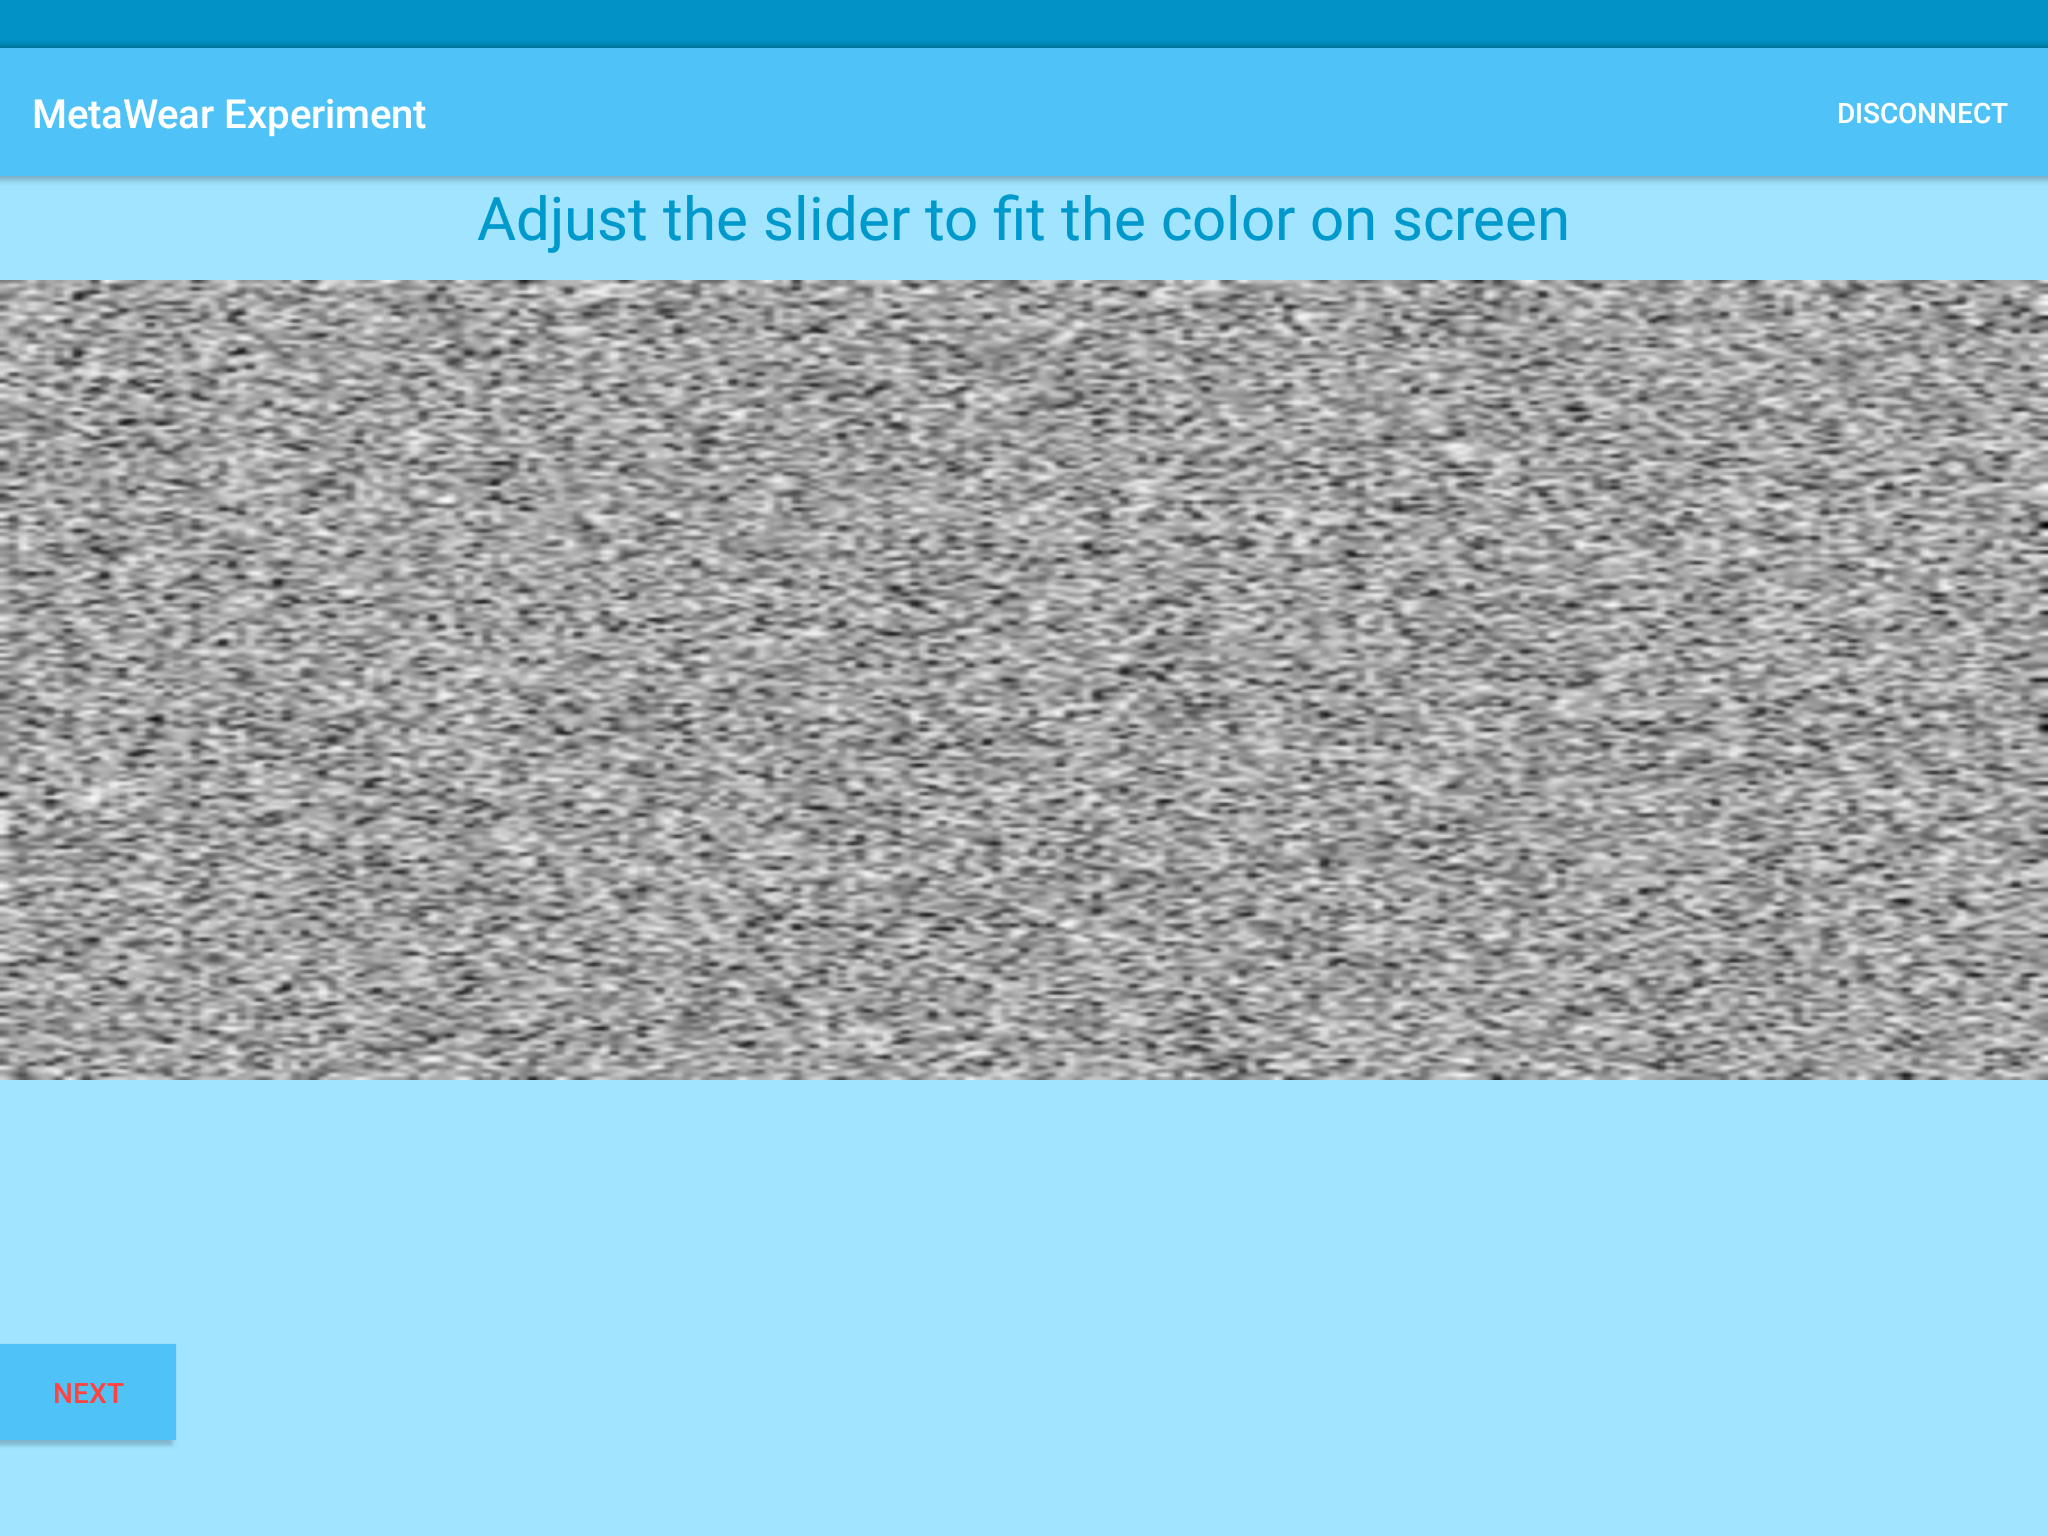
\includegraphics[width=0.9\textwidth]{figures/tablet_screen9.png}
\caption{CAPTIONBLABLA}
\label{appendix_app_screen_9}
\end{figure}

\begin{figure}[h!]
\centering
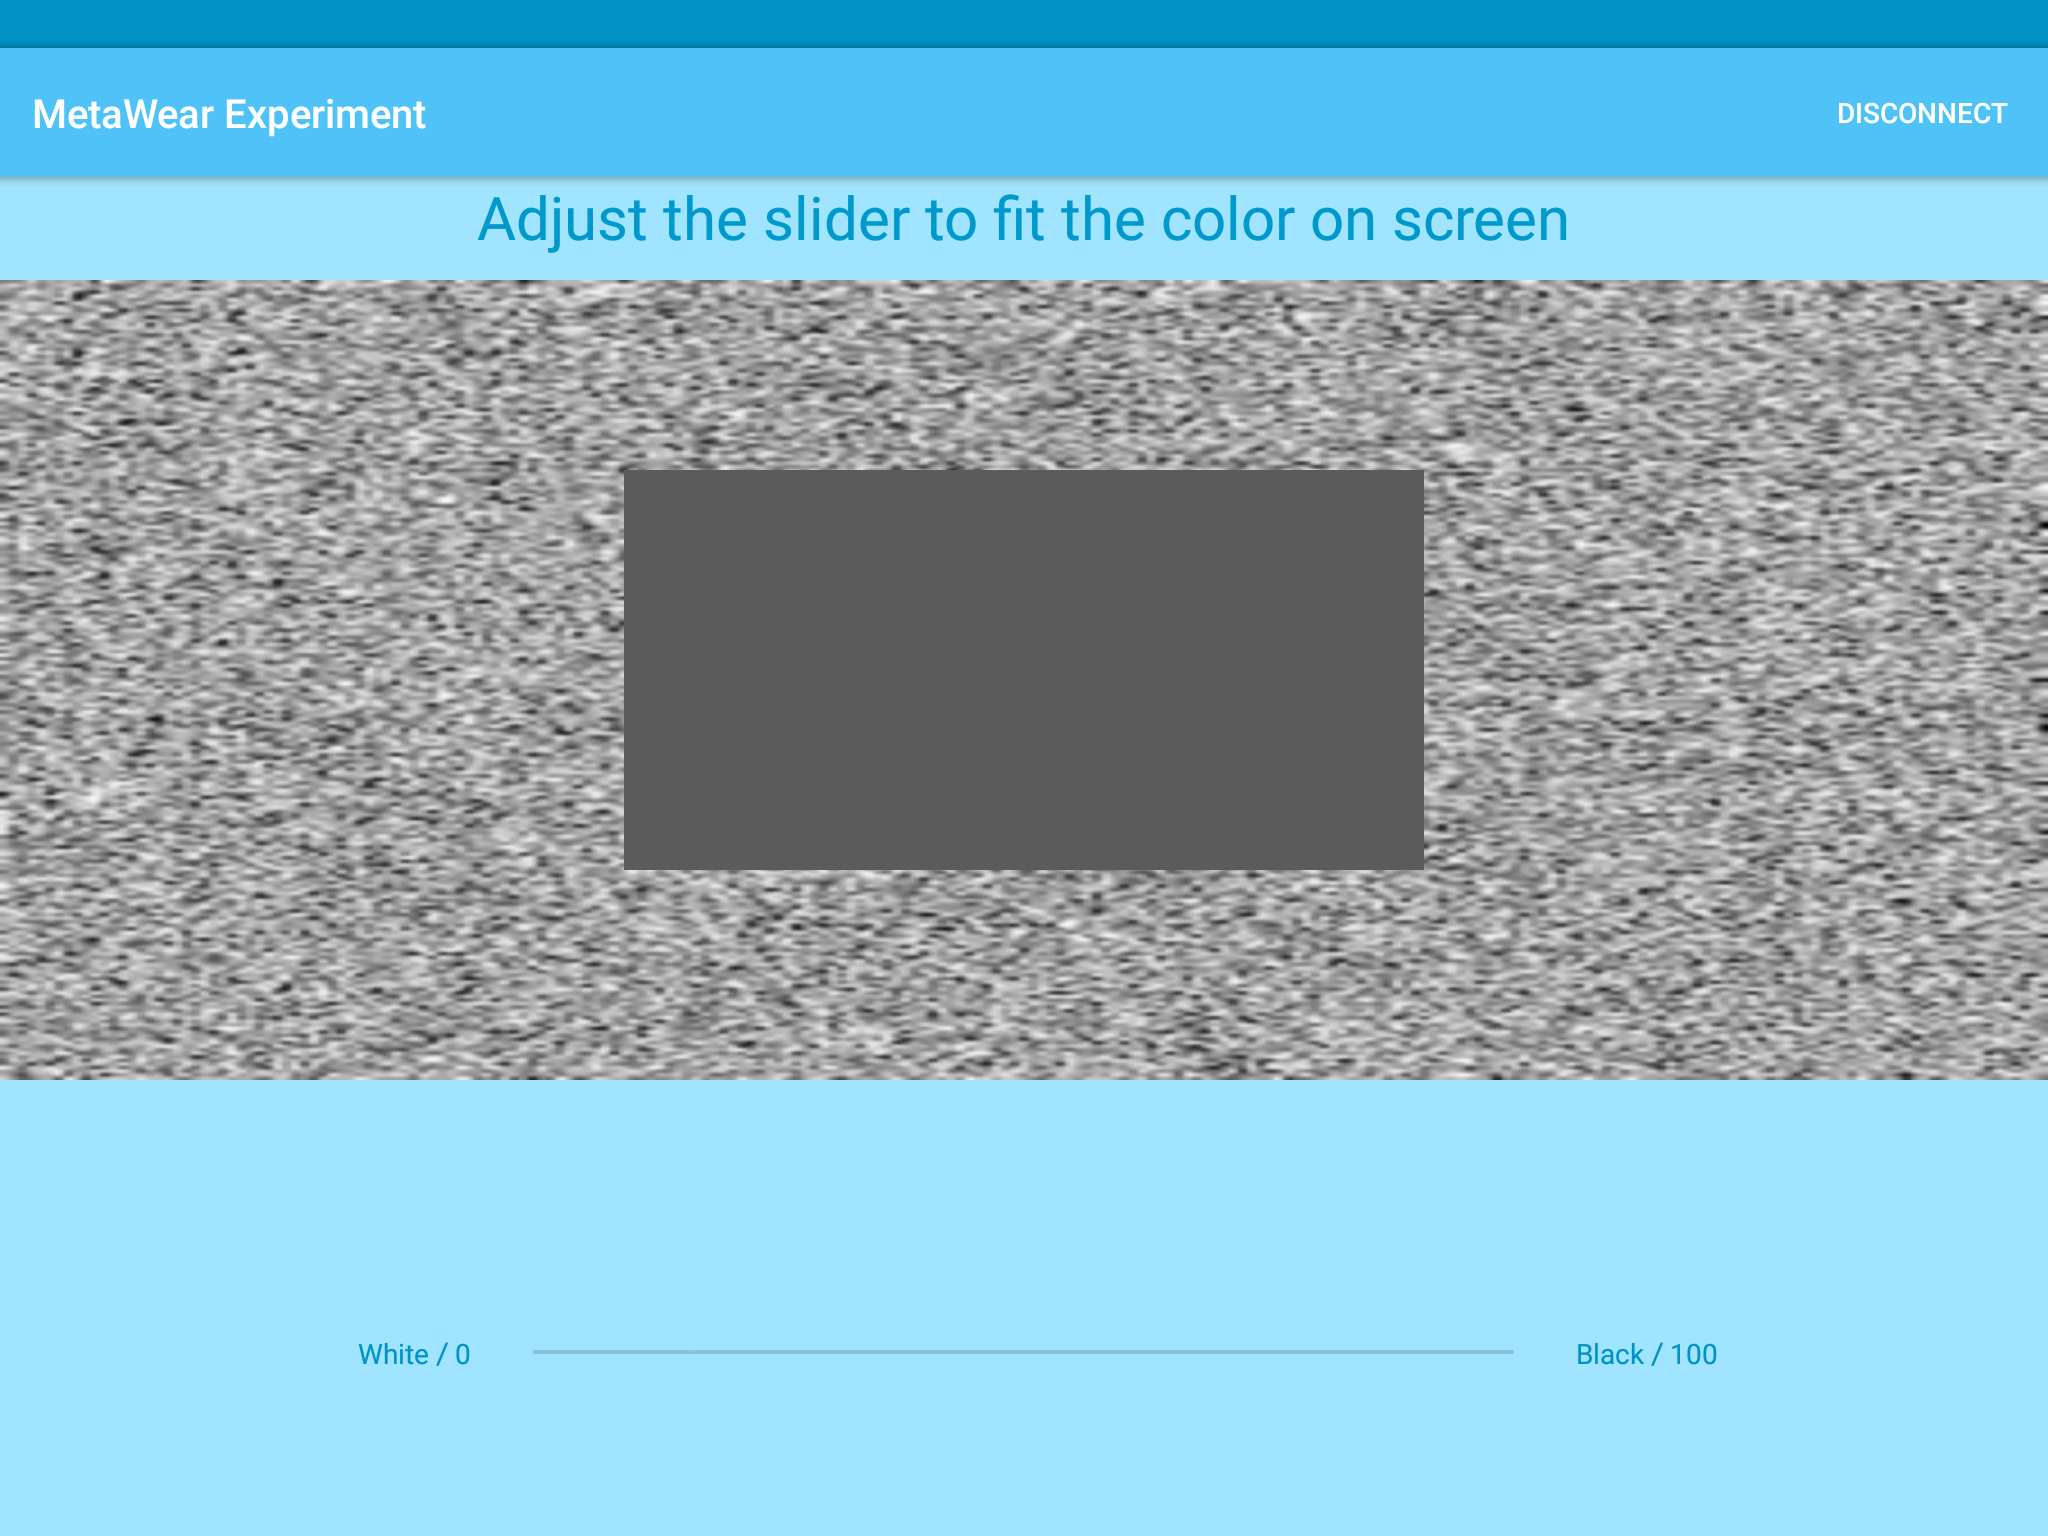
\includegraphics[width=0.9\textwidth]{figures/tablet_screen10.png}
\caption{CAPTIONBLABLA}
\label{appendix_app_screen_10}
\end{figure}

\begin{figure}[h!]
\centering
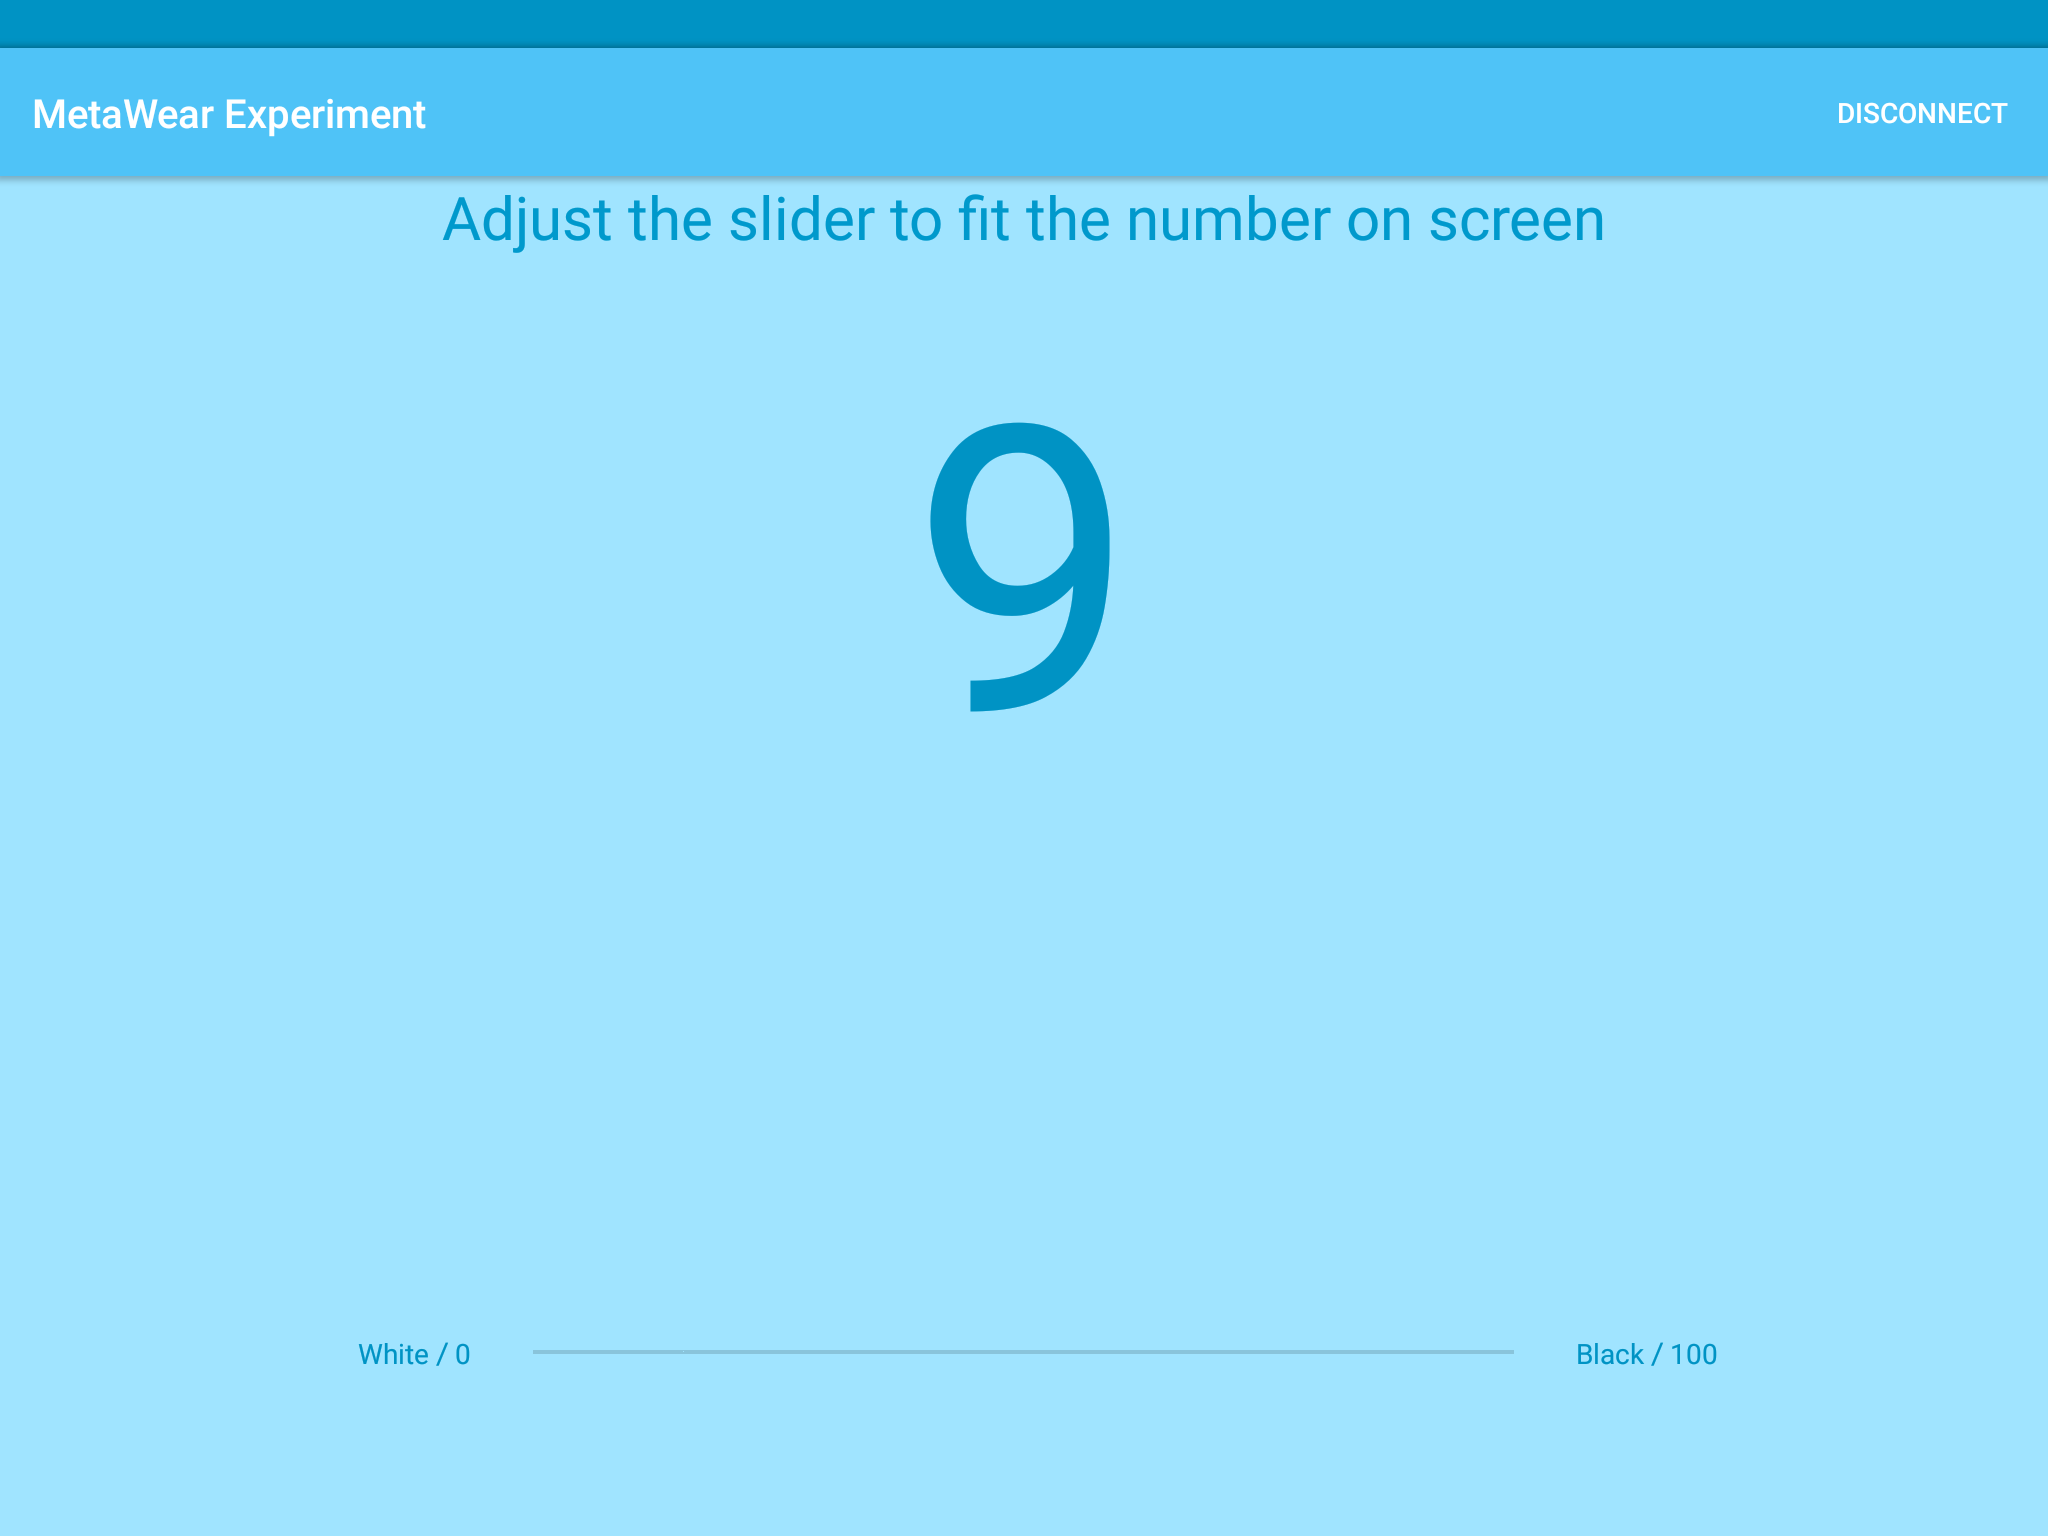
\includegraphics[width=0.9\textwidth]{figures/tablet_screen11.png}
\caption{CAPTIONBLABLA}
\label{appendix_app_screen_11}
\end{figure}

\begin{figure}[h!]
\centering
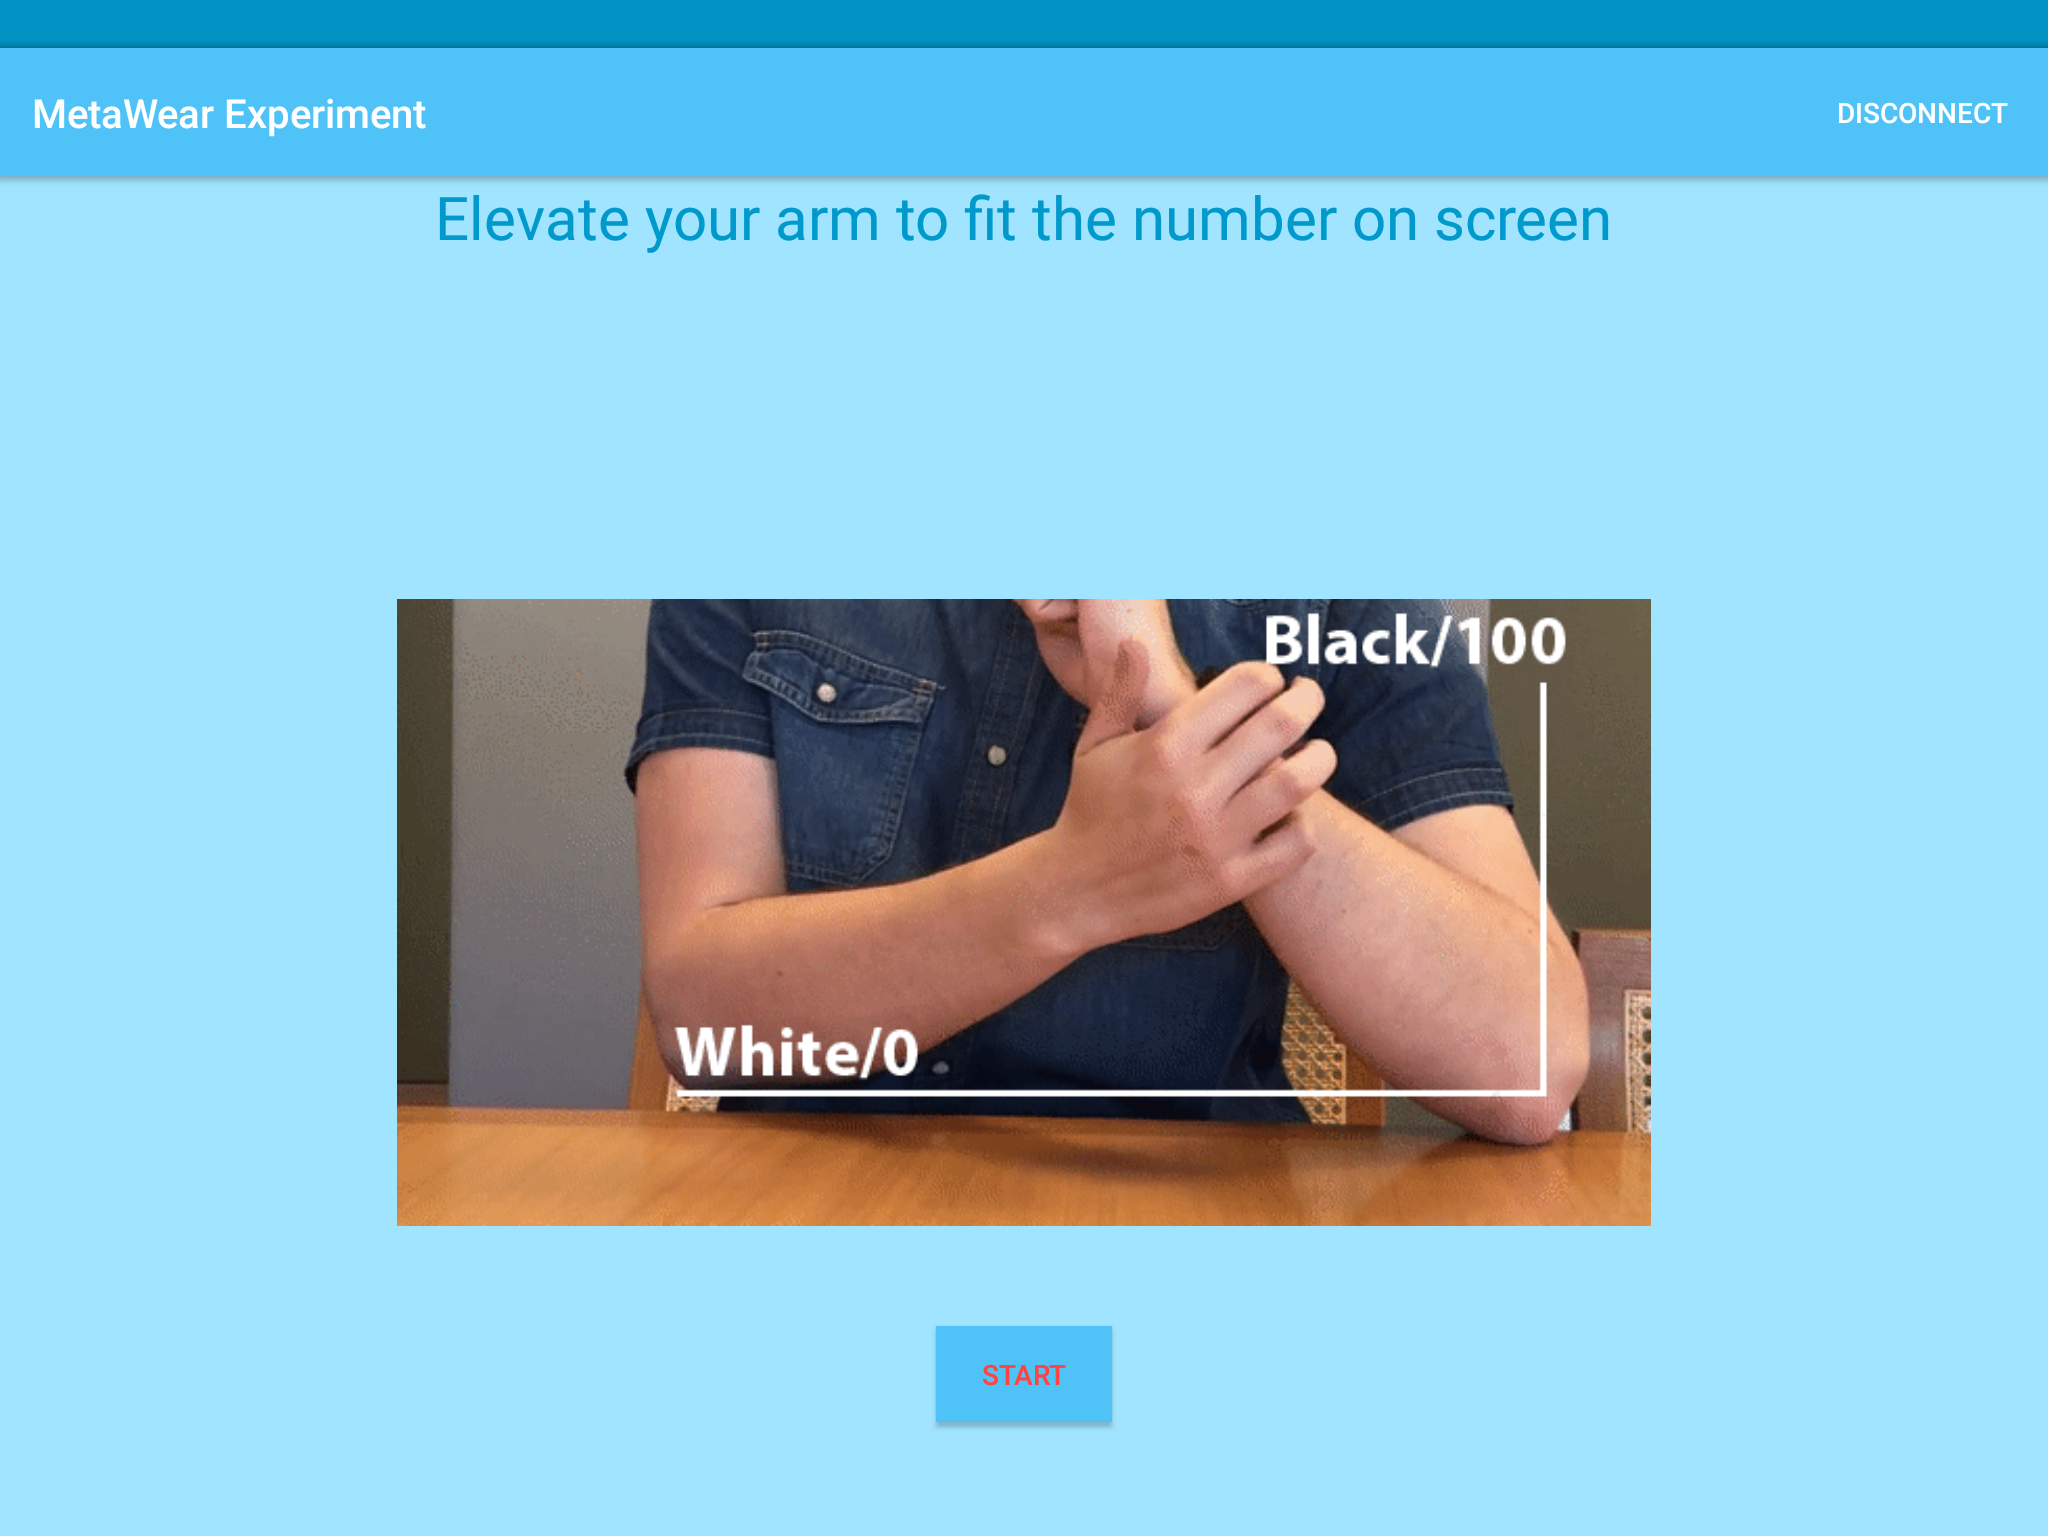
\includegraphics[width=0.9\textwidth]{figures/tablet_screen12.png}
\caption{CAPTIONBLABLA}
\label{appendix_app_screen_12}
\end{figure}

\begin{figure}[h!]
\centering
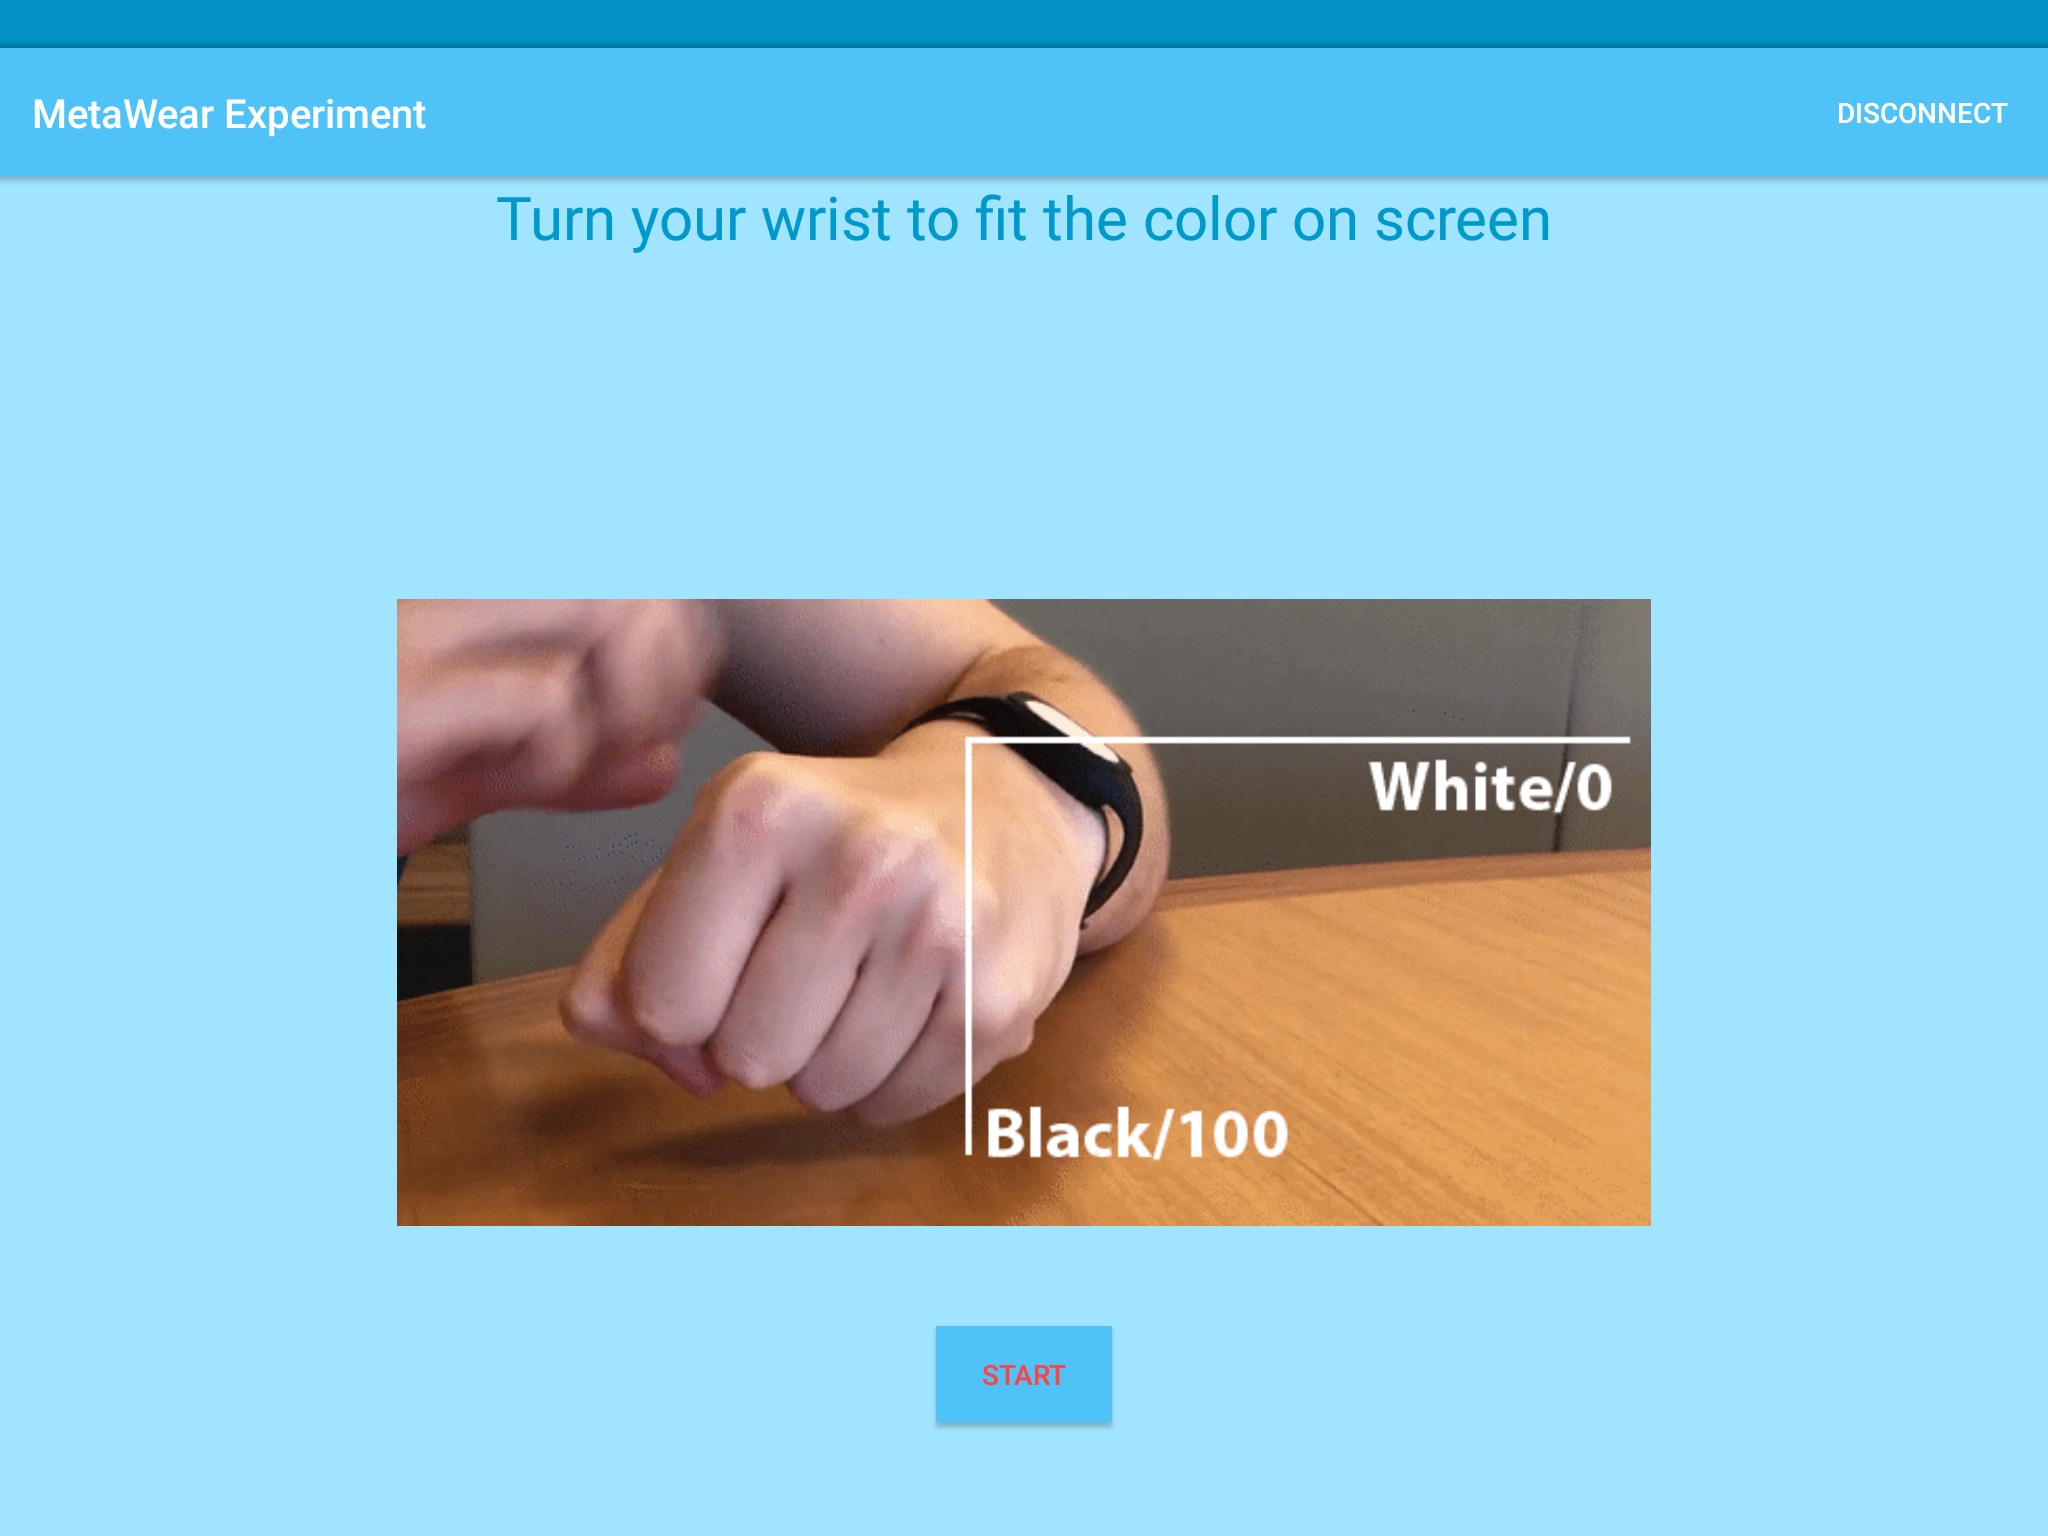
\includegraphics[width=0.9\textwidth]{figures/tablet_screen13.png}
\caption{CAPTIONBLABLA}
\label{appendix_app_screen_13}
\end{figure}

\begin{figure}[h!]
\centering
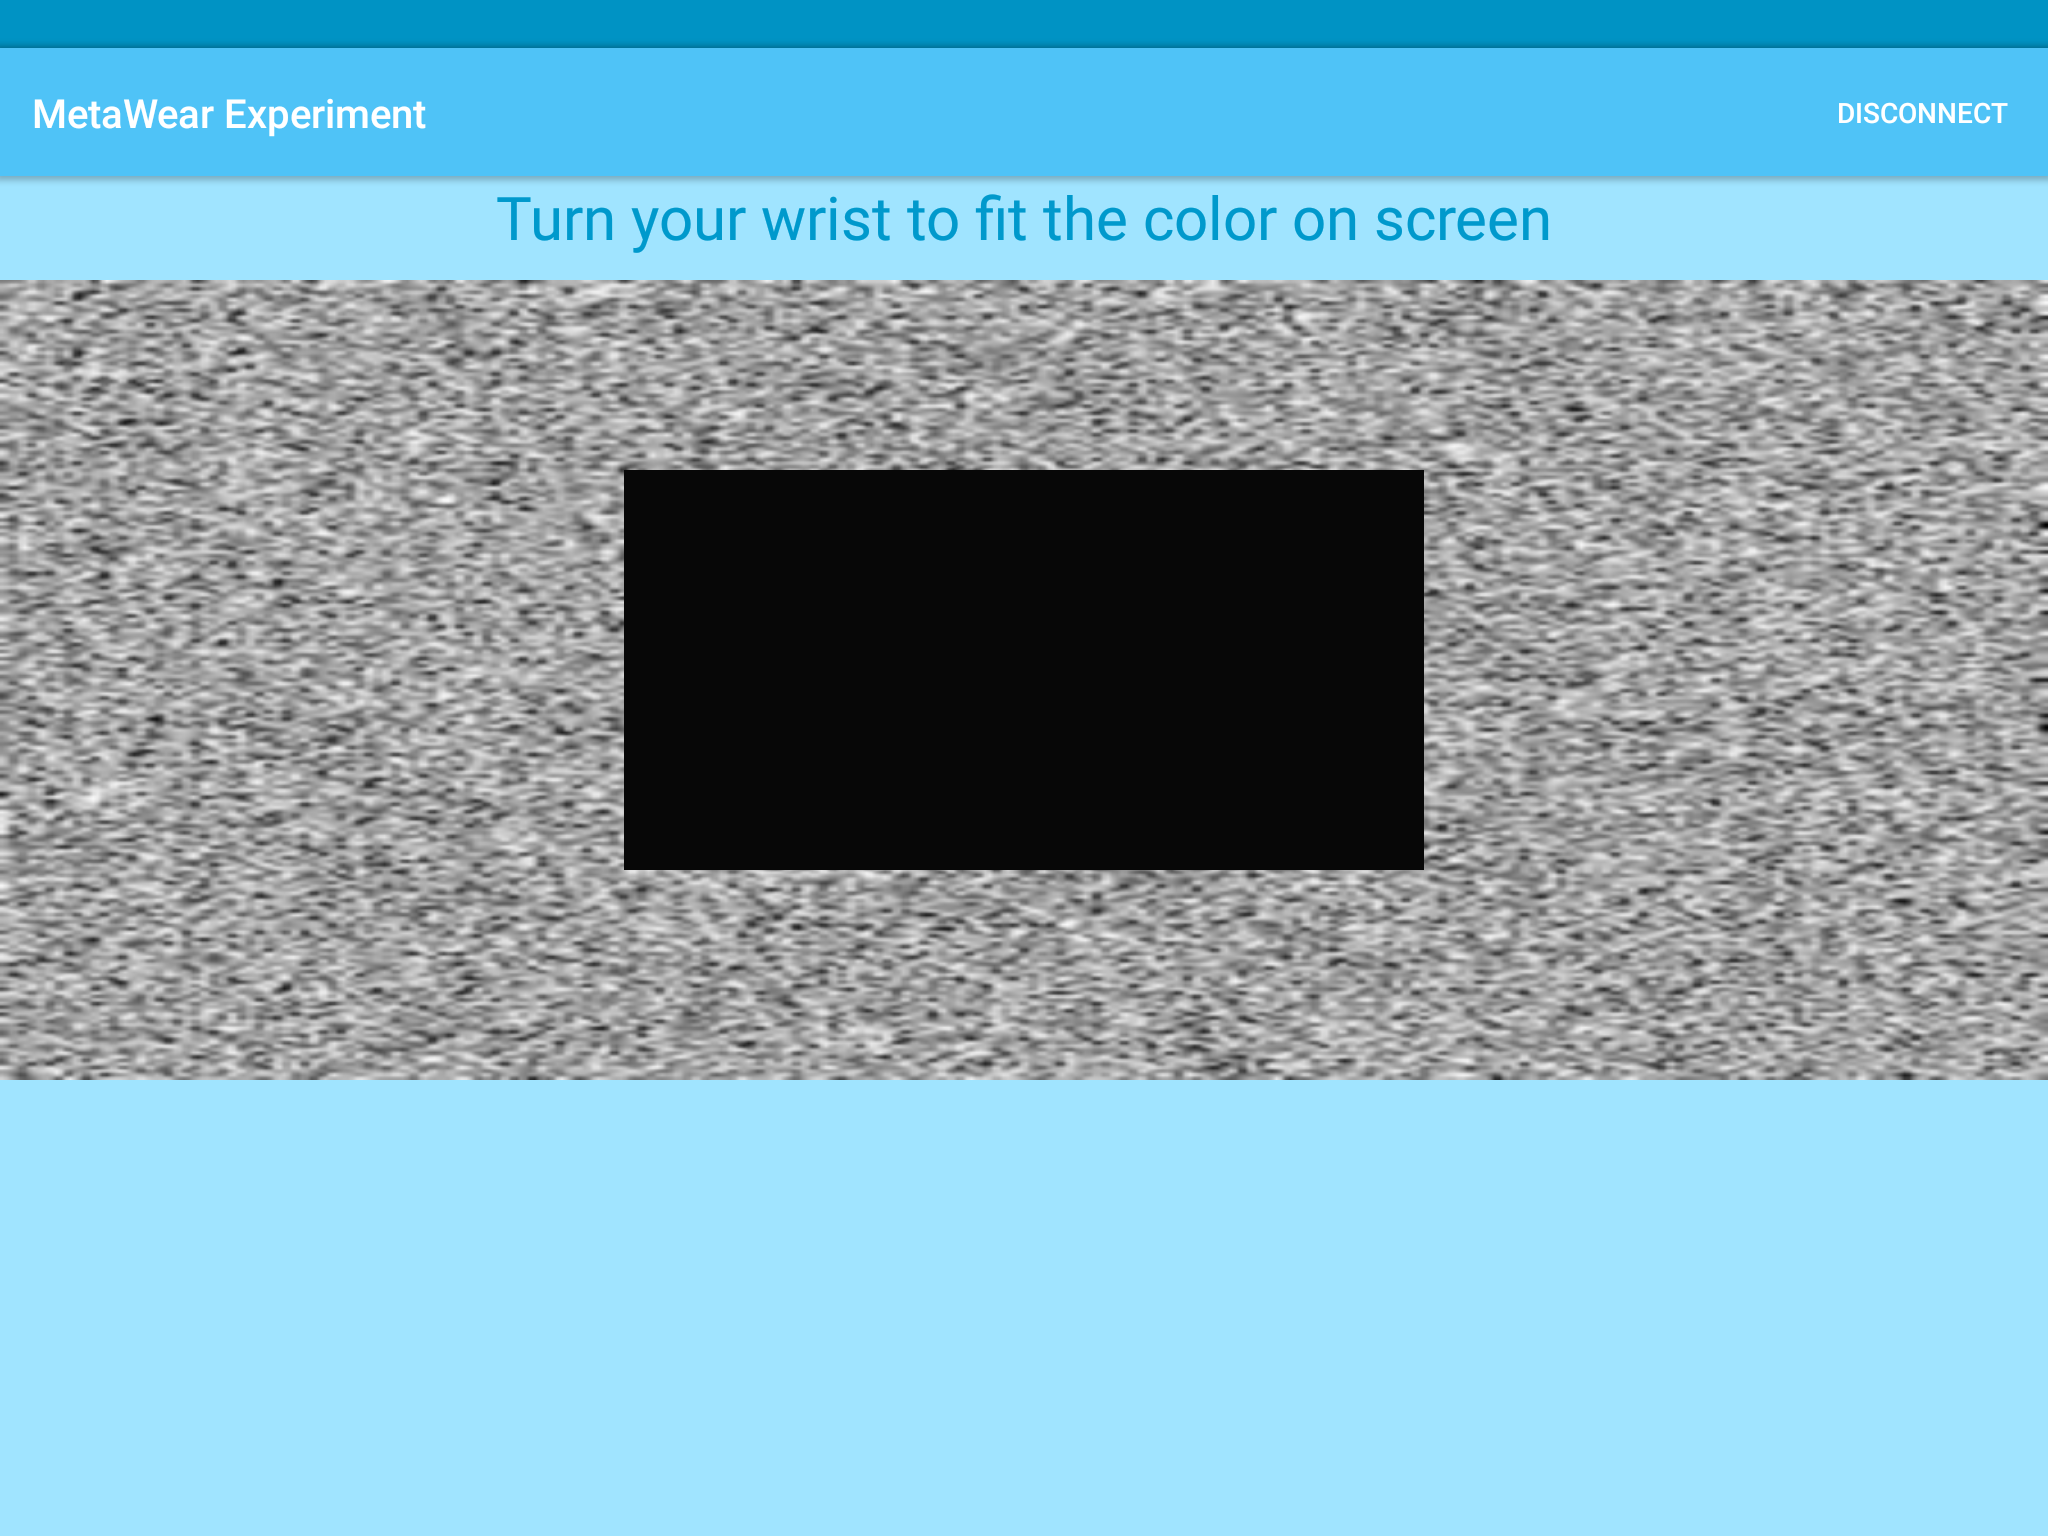
\includegraphics[width=0.9\textwidth]{figures/tablet_screen14.png}
\caption{CAPTIONBLABLA}
\label{appendix_app_screen_14}
\end{figure}

\begin{figure}[h!]
\centering
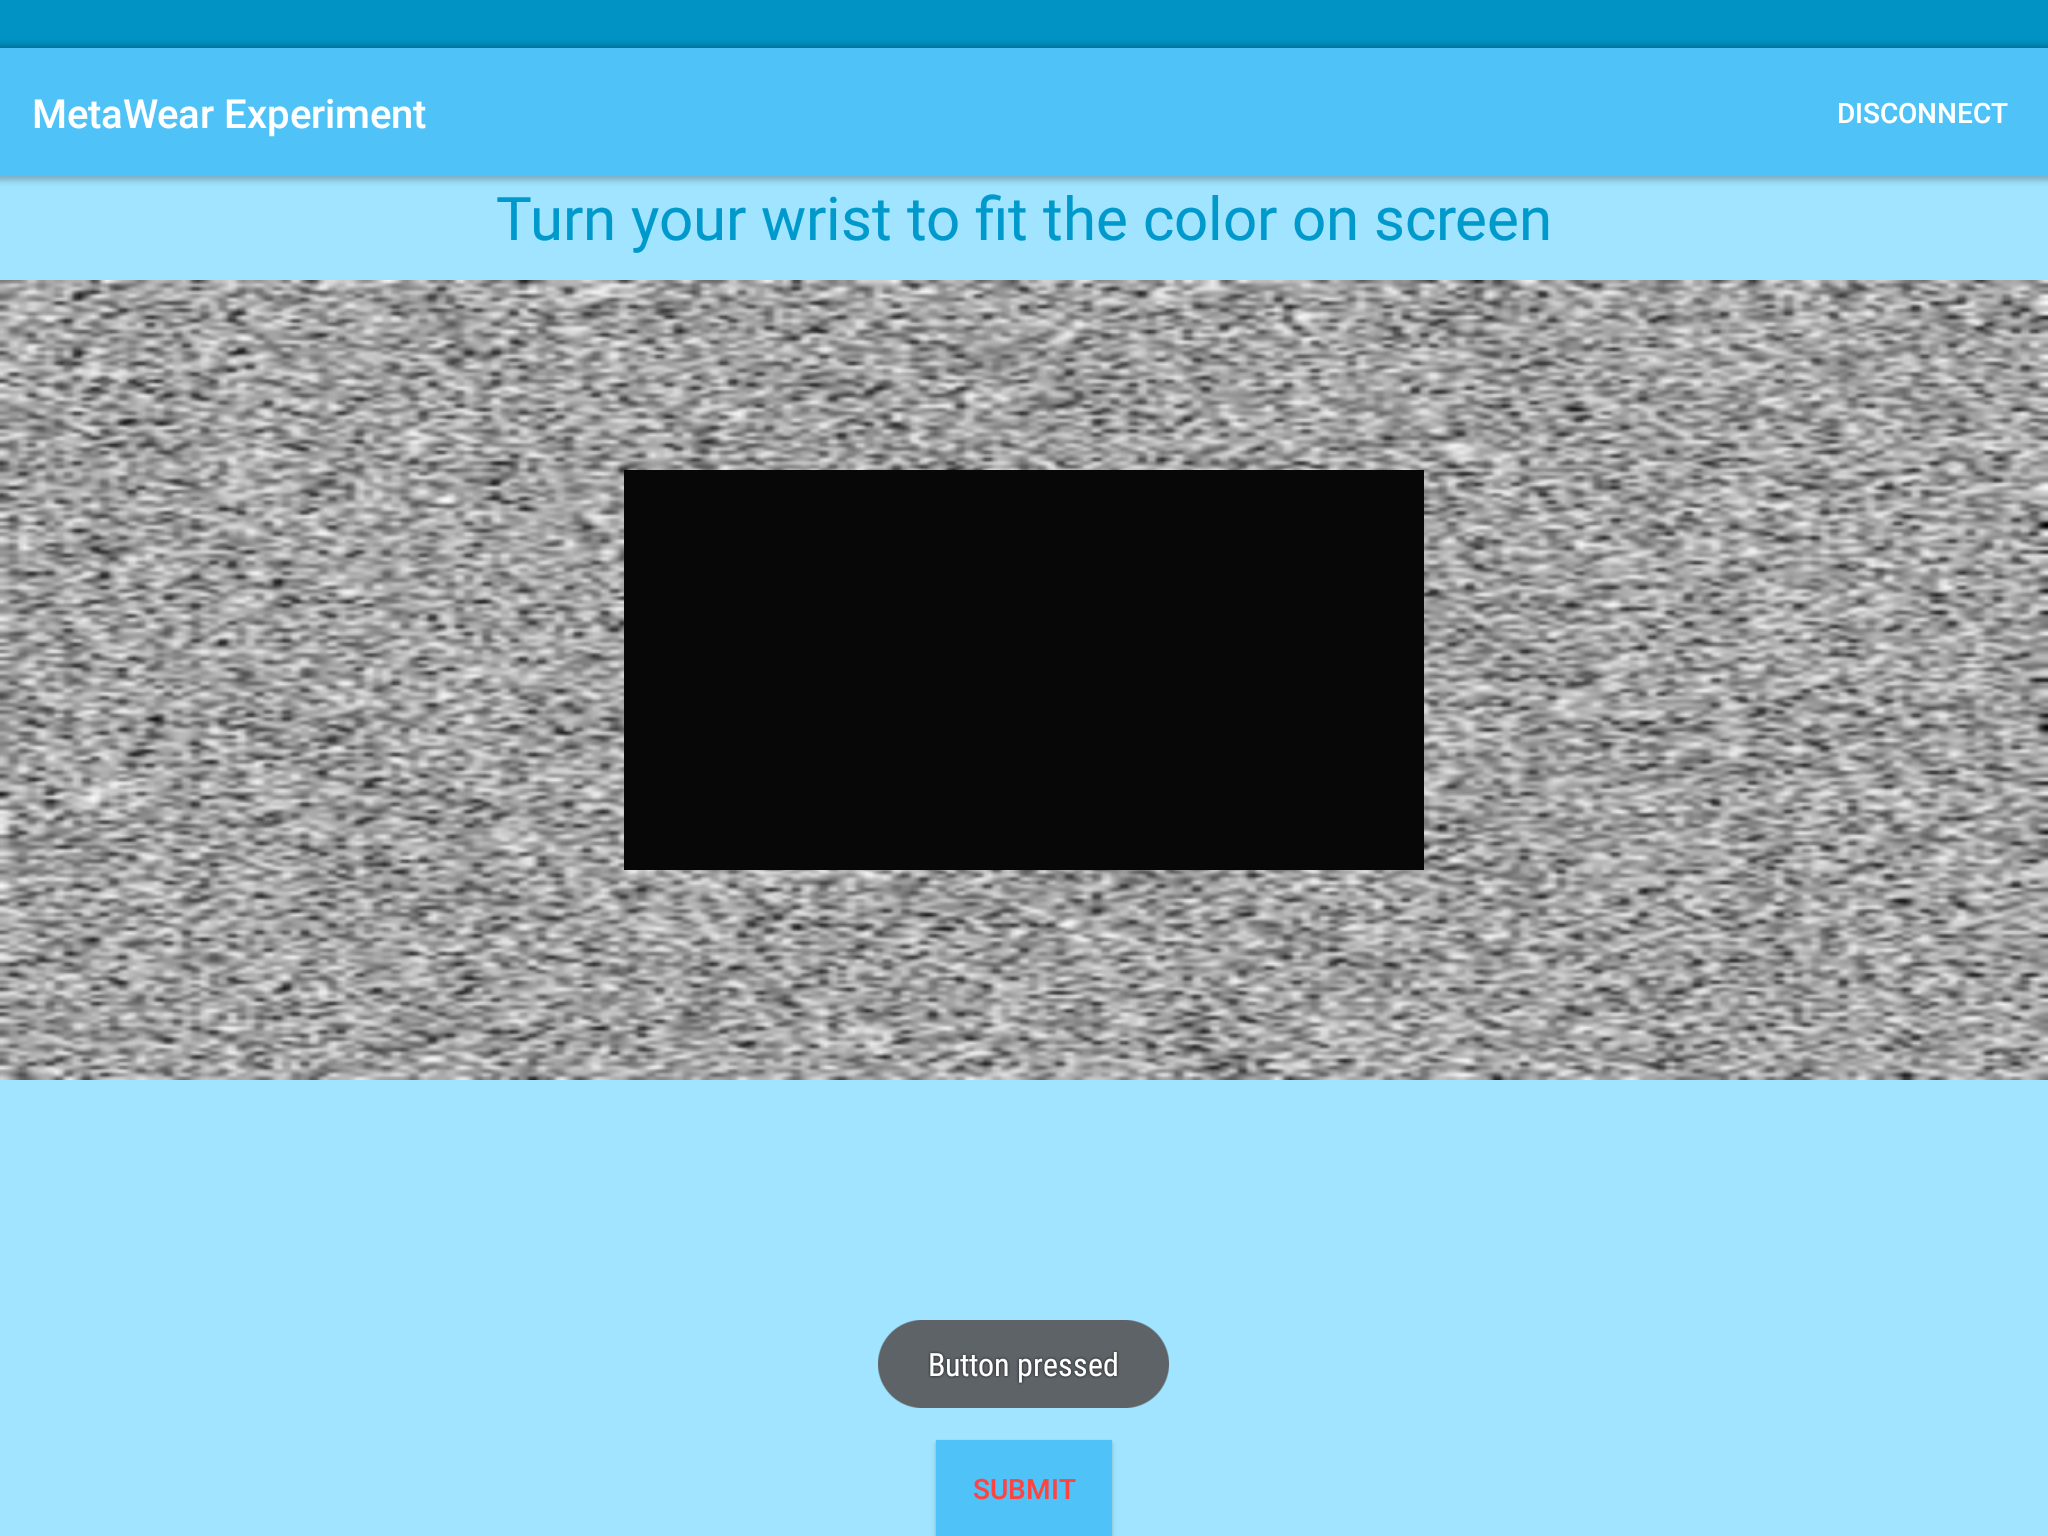
\includegraphics[width=0.9\textwidth]{figures/tablet_screen15.png}
\caption{CAPTIONBLABLA}
\label{appendix_app_screen_15}
\end{figure}

\begin{figure}[h!]
\centering
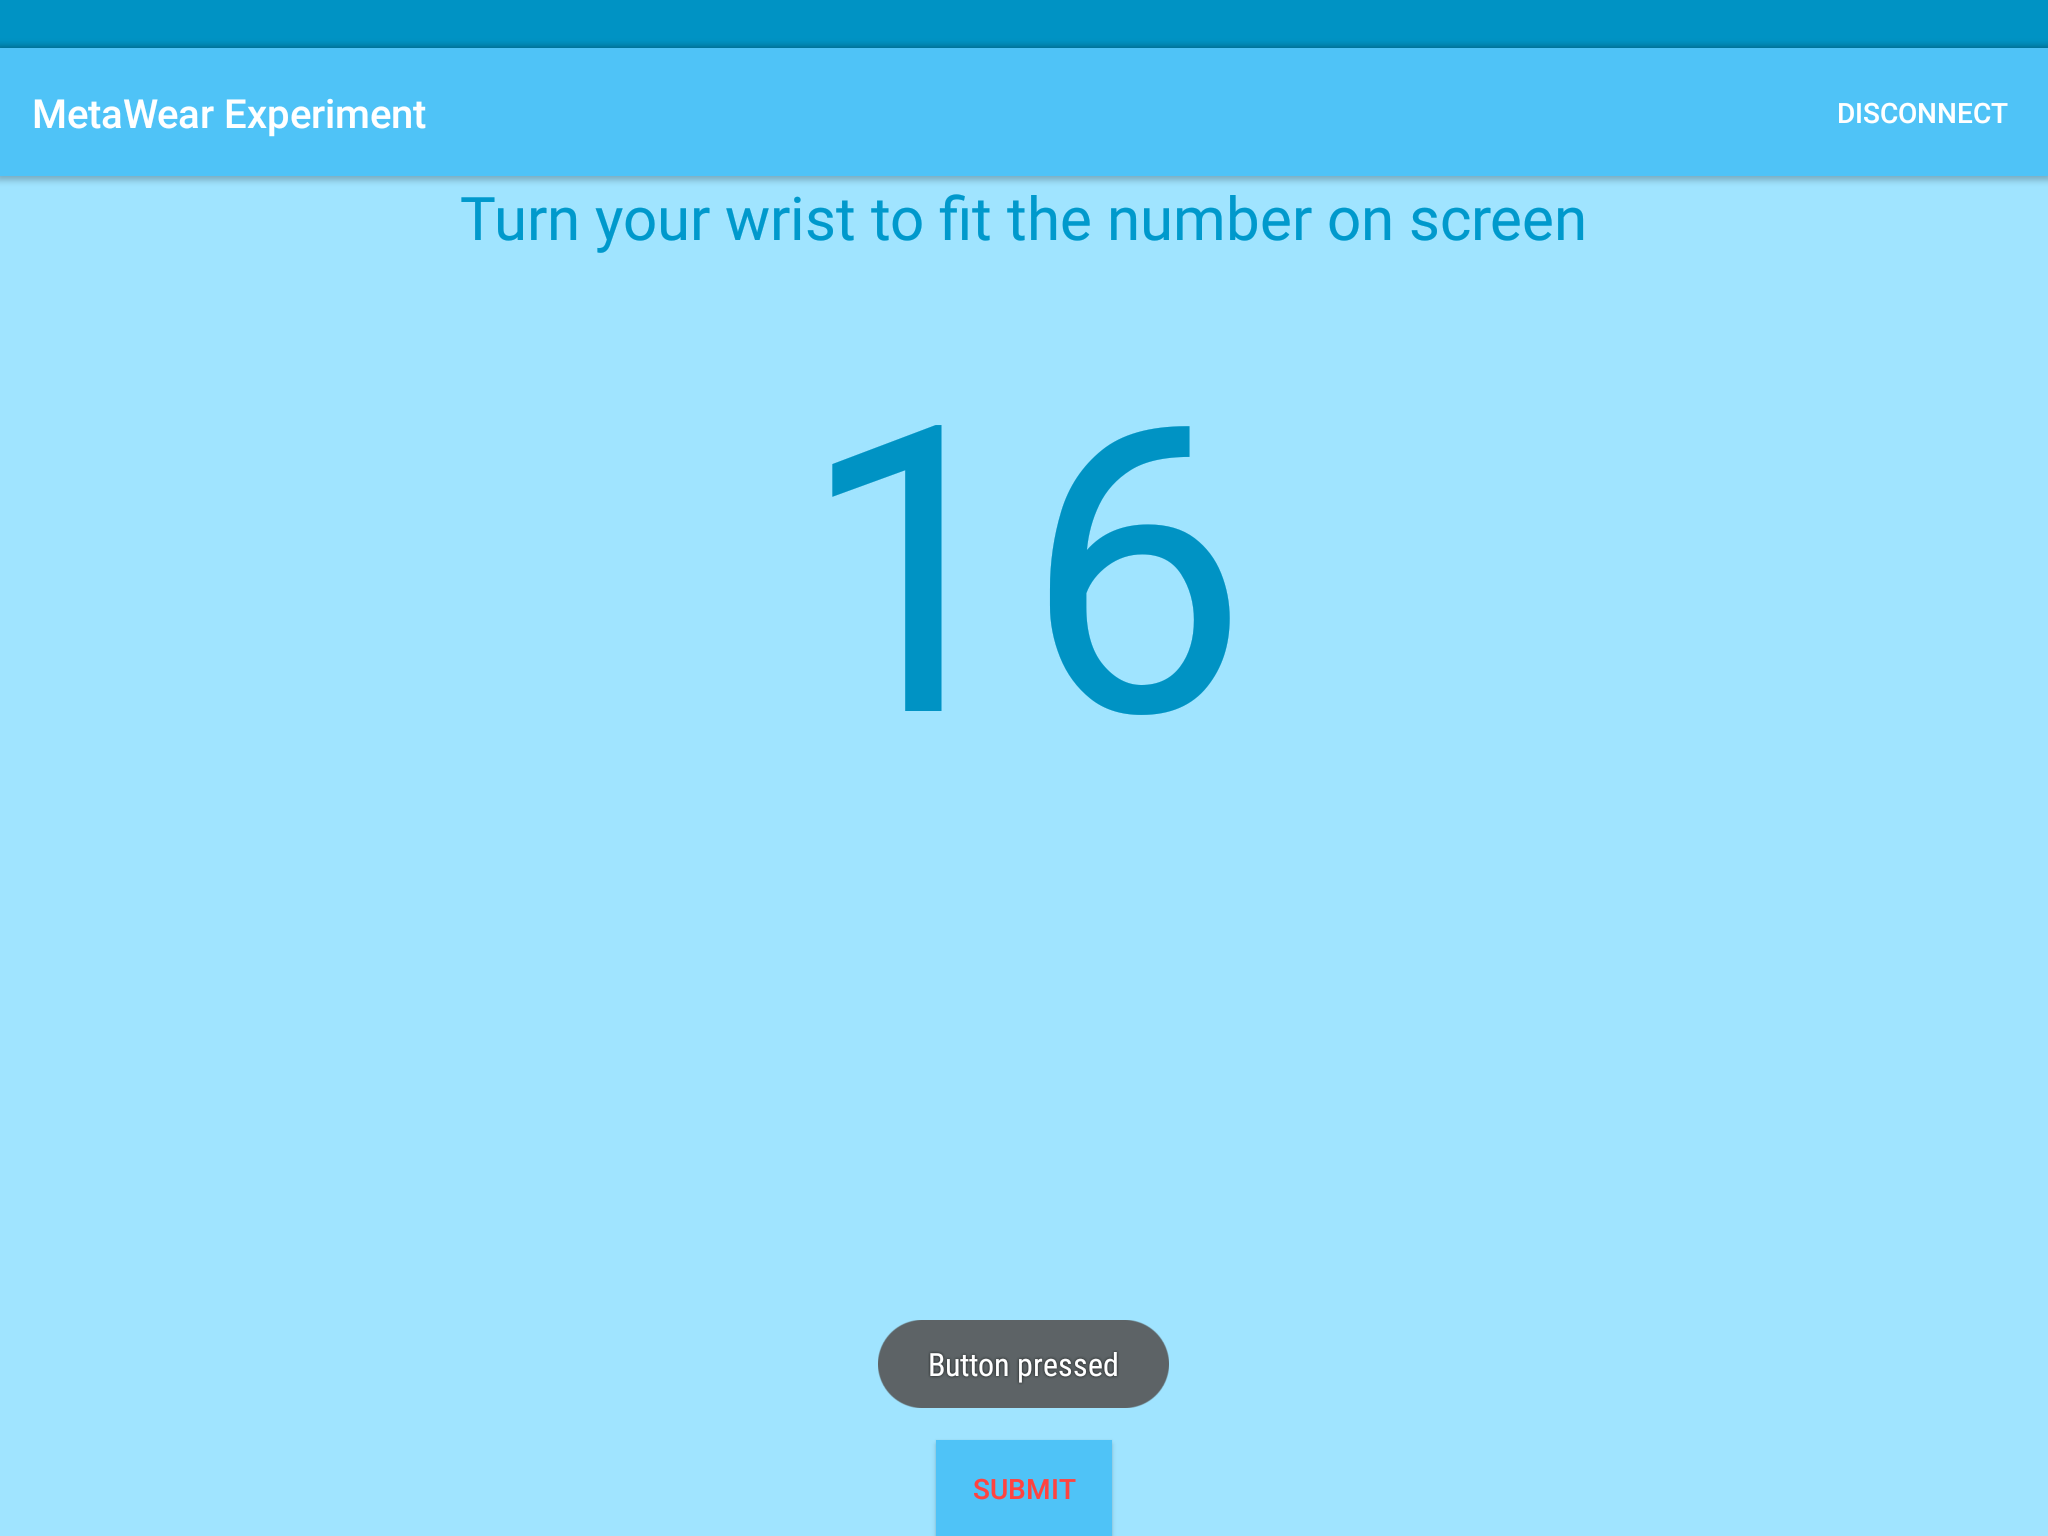
\includegraphics[width=0.9\textwidth]{figures/tablet_screen16.png}
\caption{CAPTIONBLABLA}
\label{appendix_app_screen_16}
\end{figure}

\begin{figure}[h!]
\centering
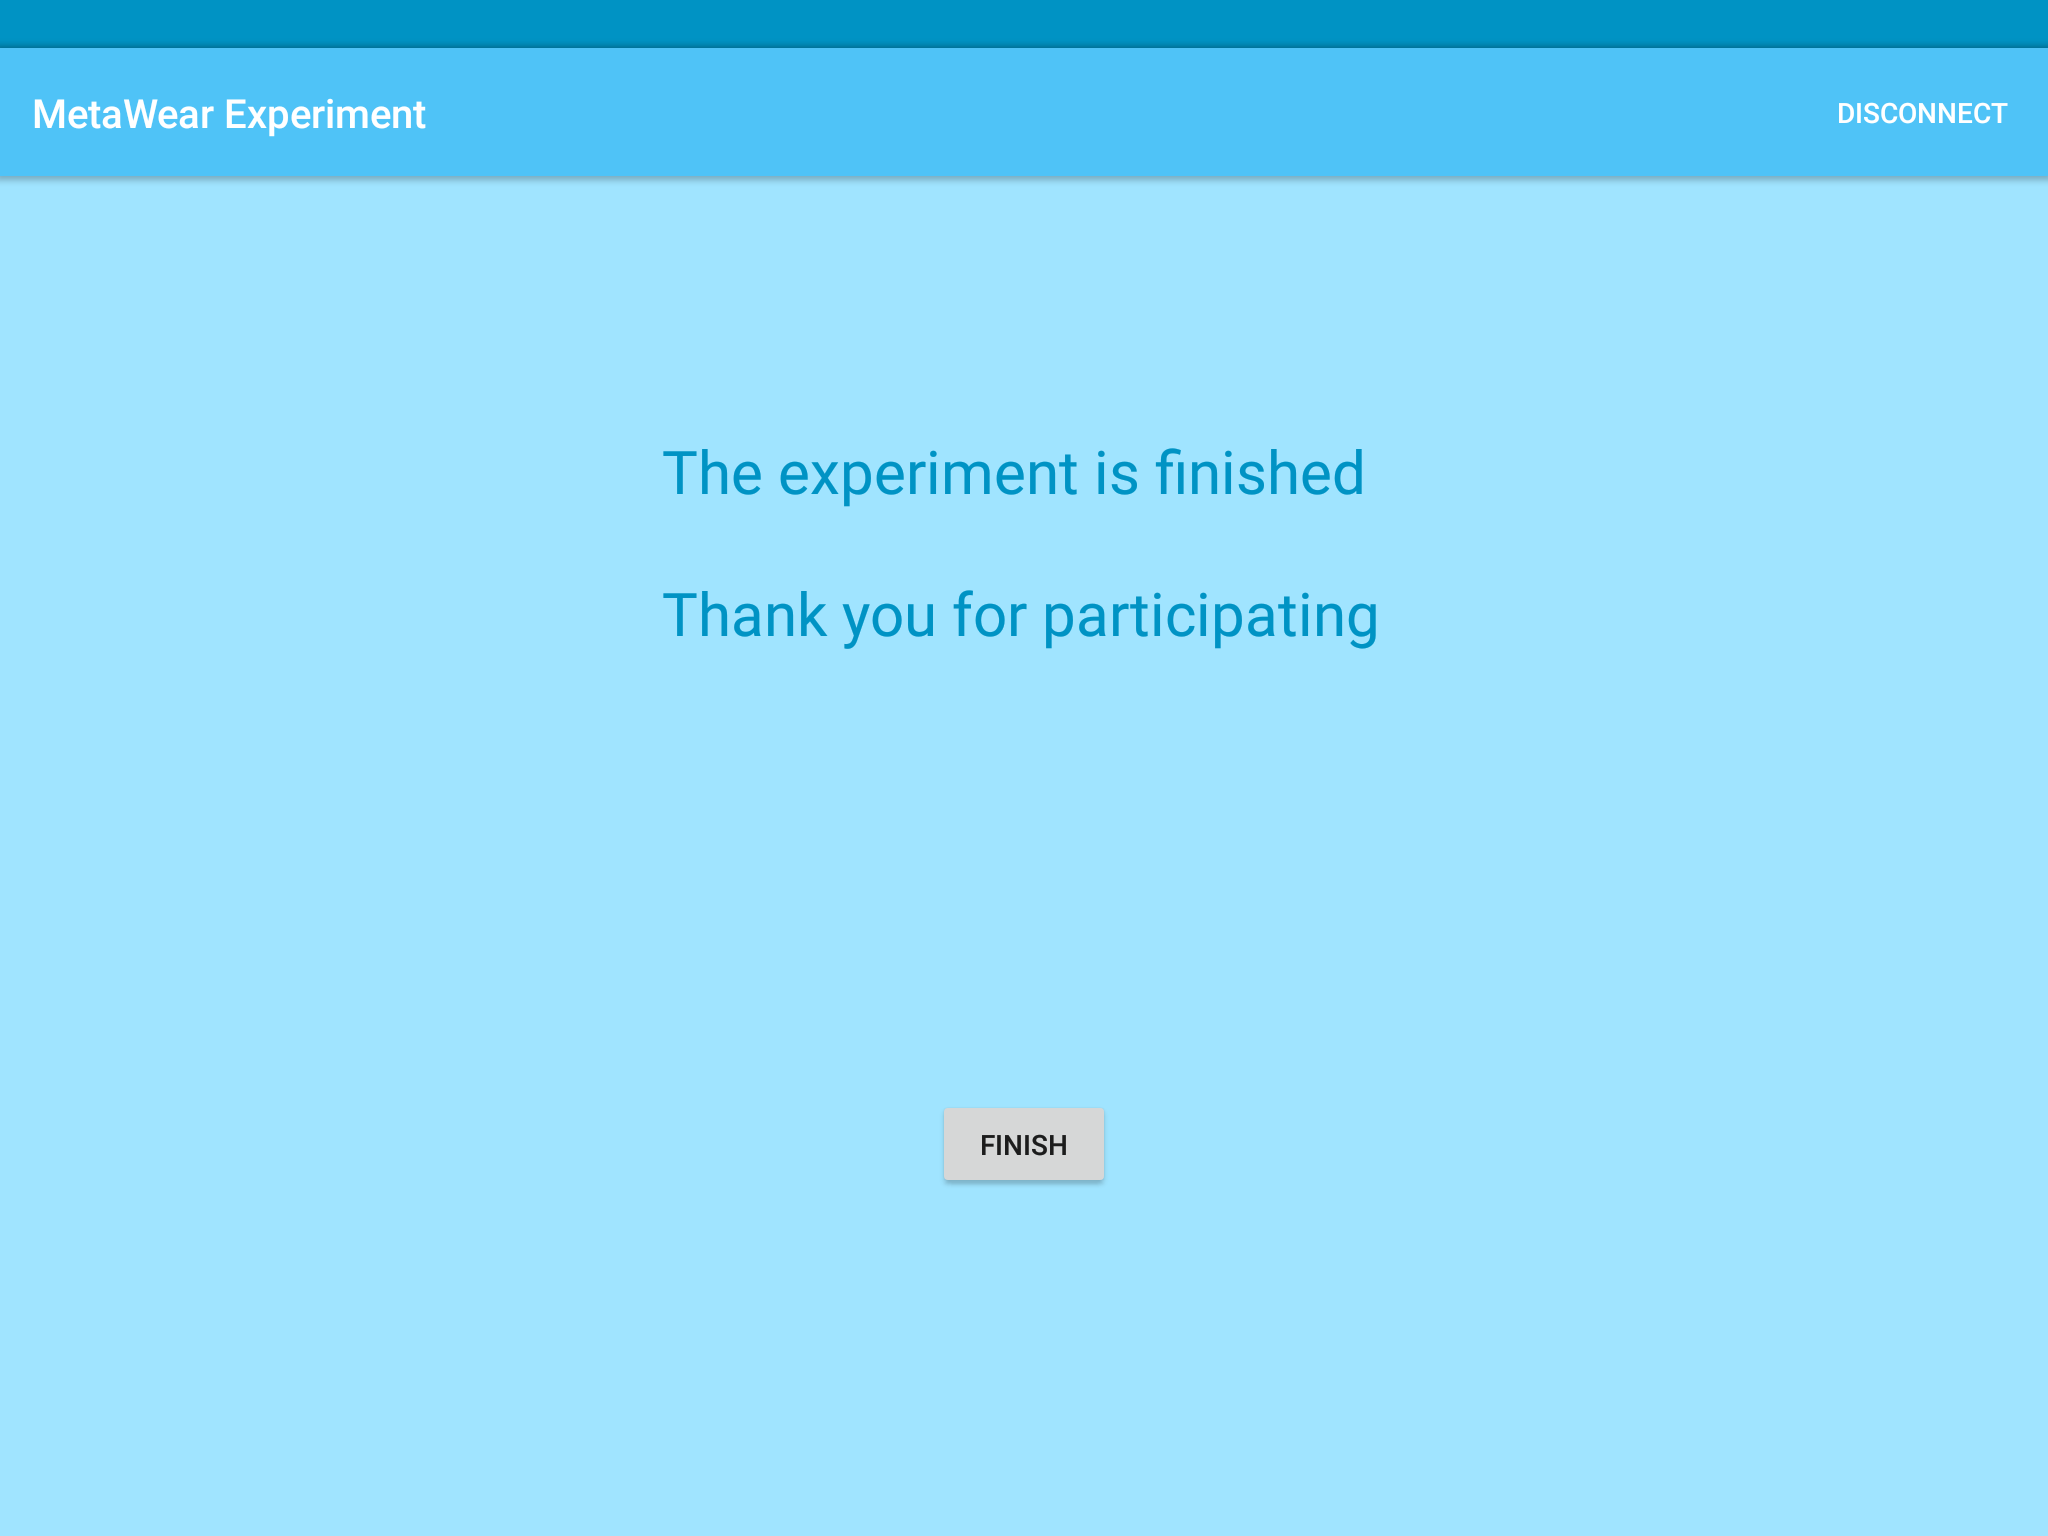
\includegraphics[width=0.9\textwidth]{figures/tablet_screen17.png}
\caption{CAPTIONBLABLA}
\label{appendix_app_screen_17}
\end{figure}

\begin{figure}[h!]
\centering
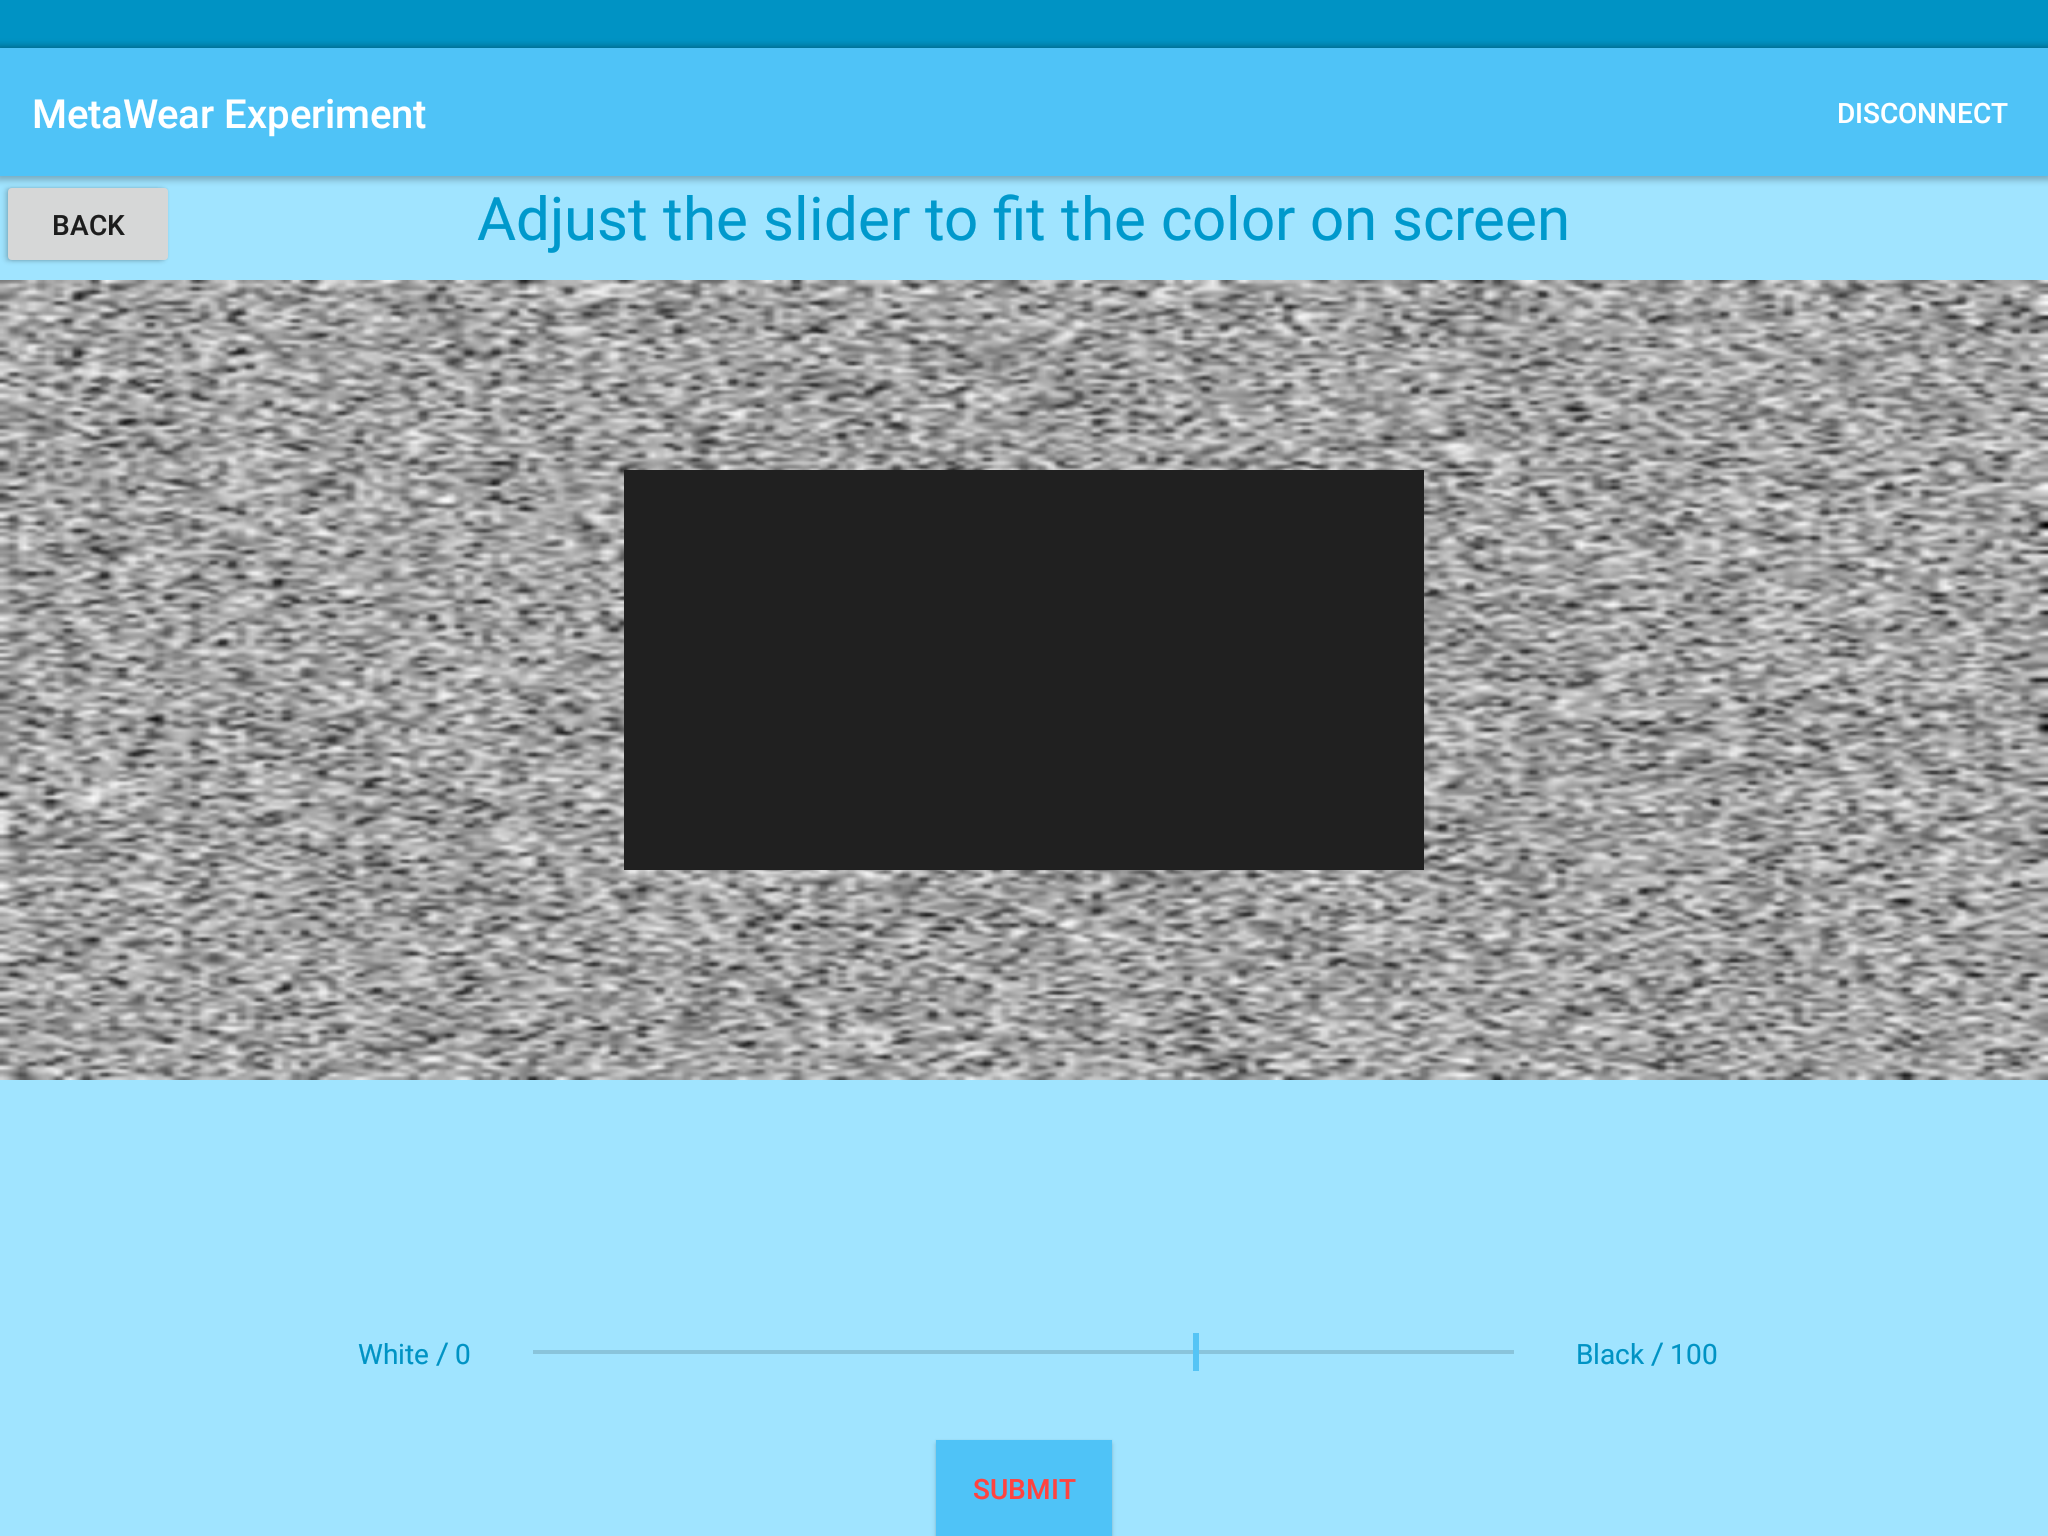
\includegraphics[width=0.9\textwidth]{figures/tablet_screen18.png}
\caption{CAPTIONBLABLA}
\label{appendix_app_screen_18}
\end{figure}